\documentclass[a4paper]{article}

\def\npart {IB}
\def\nterm {Lent}
\def\nyear {2016}
\def\nlecturer {I. Smith}
\def\ncourse {Complex Analysis}
\def\nlectures {MWF.11}
\def\nnotready {}

% Imports
\ifx \nextra \undefined
  \usepackage[pdftex,
    hidelinks,
    pdfauthor={Dexter Chua},
    pdfsubject={Cambridge Maths Notes: Part \npart\ - \ncourse},
    pdftitle={Part \npart\ - \ncourse},
  pdfkeywords={Cambridge Mathematics Maths Math \npart\ \nterm\ \nyear\ \ncourse}]{hyperref}
  \title{Part \npart\ - \ncourse}
\else
  \usepackage[pdftex,
    hidelinks,
    pdfauthor={Dexter Chua},
    pdfsubject={Cambridge Maths Notes: Part \npart\ - \ncourse\ (\nextra)},
    pdftitle={Part \npart\ - \ncourse\ (\nextra)},
  pdfkeywords={Cambridge Mathematics Maths Math \npart\ \nterm\ \nyear\ \ncourse\ \nextra}]{hyperref}

  \title{Part \npart\ - \ncourse \\ {\Large \nextra}}
\fi

\author{Lectured by \nlecturer \\\small Notes taken by Dexter Chua}
\date{\nterm\ \nyear}

\usepackage{alltt}
\usepackage{amsfonts}
\usepackage{amsmath}
\usepackage{amssymb}
\usepackage{amsthm}
\usepackage{booktabs}
\usepackage{caption}
\usepackage{enumitem}
\usepackage{fancyhdr}
\usepackage{graphicx}
\usepackage{mathtools}
\usepackage{microtype}
\usepackage{multirow}
\usepackage{pdflscape}
\usepackage{pgfplots}
\usepackage{siunitx}
\usepackage{tabularx}
\usepackage{tikz}
\usepackage{tkz-euclide}
\usepackage[normalem]{ulem}
\usepackage[all]{xy}

\pgfplotsset{compat=1.12}

\pagestyle{fancyplain}
\lhead{\emph{\nouppercase{\leftmark}}}
\ifx \nextra \undefined
  \rhead{
    \ifnum\thepage=1
    \else
      \npart\ \ncourse
    \fi}
\else
  \rhead{
    \ifnum\thepage=1
    \else
      \npart\ \ncourse\ (\nextra)
    \fi}
\fi
\usetikzlibrary{arrows}
\usetikzlibrary{decorations.markings}
\usetikzlibrary{decorations.pathmorphing}
\usetikzlibrary{positioning}
\usetikzlibrary{fadings}
\usetikzlibrary{intersections}
\usetikzlibrary{cd}

\newcommand*{\Cdot}{\raisebox{-0.25ex}{\scalebox{1.5}{$\cdot$}}}
\newcommand {\pd}[2][ ]{
  \ifx #1 { }
    \frac{\partial}{\partial #2}
  \else
    \frac{\partial^{#1}}{\partial #2^{#1}}
  \fi
}

% Theorems
\theoremstyle{definition}
\newtheorem*{aim}{Aim}
\newtheorem*{axiom}{Axiom}
\newtheorem*{claim}{Claim}
\newtheorem*{cor}{Corollary}
\newtheorem*{defi}{Definition}
\newtheorem*{eg}{Example}
\newtheorem*{fact}{Fact}
\newtheorem*{law}{Law}
\newtheorem*{lemma}{Lemma}
\newtheorem*{notation}{Notation}
\newtheorem*{prop}{Proposition}
\newtheorem*{thm}{Theorem}

\renewcommand{\labelitemi}{--}
\renewcommand{\labelitemii}{$\circ$}
\renewcommand{\labelenumi}{(\roman{*})}

\let\stdsection\section
\renewcommand\section{\newpage\stdsection}

% Strike through
\def\st{\bgroup \ULdepth=-.55ex \ULset}

% Maths symbols
\newcommand{\bra}{\langle}
\newcommand{\ket}{\rangle}

\newcommand{\N}{\mathbb{N}}
\newcommand{\Z}{\mathbb{Z}}
\newcommand{\Q}{\mathbb{Q}}
\renewcommand{\H}{\mathbb{H}}
\newcommand{\R}{\mathbb{R}}
\newcommand{\C}{\mathbb{C}}
\newcommand{\Prob}{\mathbb{P}}
\renewcommand{\P}{\mathbb{P}}
\newcommand{\E}{\mathbb{E}}
\newcommand{\F}{\mathbb{F}}
\newcommand{\cU}{\mathcal{U}}
\newcommand{\RP}{\mathbb{RP}}
\newcommand{\CP}{\mathbb{CP}}

\newcommand{\ph}{\,\cdot\,}

\DeclareMathOperator{\sech}{sech}
\DeclareMathOperator{\cosech}{cosech}
\DeclareMathOperator{\cosec}{cosec}

\DeclareMathOperator{\covol}{covol}
\DeclareMathOperator{\vol}{vol}

\let\Im\relax
\let\Re\relax
\DeclareMathOperator{\Im}{Im}
\DeclareMathOperator{\Re}{Re}
\DeclareMathOperator{\im}{im}
\DeclareMathOperator{\image}{image}
\DeclareMathOperator{\Ann}{Ann}

\DeclareMathOperator*{\res}{res}
\DeclareMathOperator{\Res}{Res}
\DeclareMathOperator{\Ind}{Ind}

\DeclareMathOperator{\tr}{tr}
\DeclareMathOperator{\diag}{diag}
\DeclareMathOperator{\rank}{rank}
\DeclareMathOperator{\card}{card}
\DeclareMathOperator{\spn}{span}
\DeclareMathOperator{\adj}{adj}

\DeclareMathOperator{\erf}{erf}
\DeclareMathOperator{\erfc}{erfc}

\DeclareMathOperator{\ord}{ord}
\DeclareMathOperator{\Sym}{Sym}

\DeclareMathOperator{\sgn}{sgn}
\DeclareMathOperator{\orb}{orb}
\DeclareMathOperator{\stab}{stab}
\DeclareMathOperator{\ccl}{ccl}

\DeclareMathOperator{\lcm}{lcm}
\DeclareMathOperator{\hcf}{hcf}

\DeclareMathOperator{\Int}{Int}
\DeclareMathOperator{\id}{id}

\DeclareMathOperator{\betaD}{beta}
\DeclareMathOperator{\gammaD}{gamma}
\DeclareMathOperator{\Poisson}{Poisson}
\DeclareMathOperator{\binomial}{binomial}
\DeclareMathOperator{\multinomial}{multinomial}
\DeclareMathOperator{\Bernoulli}{Bernoulli}
\DeclareMathOperator{\like}{like}

\DeclareMathOperator{\var}{var}
\DeclareMathOperator{\cov}{cov}
\DeclareMathOperator{\bias}{bias}
\DeclareMathOperator{\mse}{mse}
\DeclareMathOperator{\corr}{corr}

\DeclareMathOperator{\otp}{otp}
\DeclareMathOperator{\dom}{dom}

\DeclareMathOperator{\Root}{Root}
\DeclareMathOperator{\supp}{supp}
\DeclareMathOperator{\rel}{rel}
\DeclareMathOperator{\Hom}{Hom}
\DeclareMathOperator{\Aut}{Aut}
\DeclareMathOperator{\Gal}{Gal}
\DeclareMathOperator{\Mat}{Mat}
\DeclareMathOperator{\End}{End}
\DeclareMathOperator{\Char}{char}
\DeclareMathOperator{\ev}{ev}
\DeclareMathOperator{\St}{St}
\DeclareMathOperator{\Lk}{Lk}
\DeclareMathOperator{\disc}{disc}
\DeclareMathOperator{\Isom}{Isom}
\DeclareMathOperator{\length}{length}
\DeclareMathOperator{\energy}{energy}
\DeclareMathOperator{\area}{area}
\DeclareMathOperator{\Syl}{Syl}
\DeclareMathOperator{\cl}{cl}
\DeclareMathOperator{\fix}{fix}

\newcommand{\GL}{\mathrm{GL}}
\newcommand{\SL}{\mathrm{SL}}
\newcommand{\PGL}{\mathrm{PGL}}
\newcommand{\PSL}{\mathrm{PSL}}
\newcommand{\PSU}{\mathrm{PSU}}
\newcommand{\Or}{\mathrm{O}}
\newcommand{\SO}{\mathrm{SO}}
\newcommand{\U}{\mathrm{U}}
\newcommand{\SU}{\mathrm{SU}}

\renewcommand{\d}{\mathrm{d}}
\newcommand{\D}{\mathrm{D}}

\tikzset{->/.style = {decoration={markings,
                                  mark=at position 1 with {\arrow[scale=2]{latex'}}},
                      postaction={decorate}}}
\tikzset{<-/.style = {decoration={markings,
                                  mark=at position 0 with {\arrowreversed[scale=2]{latex'}}},
                      postaction={decorate}}}
\tikzset{<->/.style = {decoration={markings,
                                   mark=at position 0 with {\arrowreversed[scale=2]{latex'}},
                                   mark=at position 1 with {\arrow[scale=2]{latex'}}},
                       postaction={decorate}}}
\tikzset{->-/.style = {decoration={markings,
                                   mark=at position #1 with {\arrow[scale=2]{latex'}}},
                       postaction={decorate}}}
\tikzset{-<-/.style = {decoration={markings,
                                   mark=at position #1 with {\arrowreversed[scale=2]{latex'}}},
                       postaction={decorate}}}

\tikzset{circ/.style = {fill, circle, inner sep = 0, minimum size = 3}}
\tikzset{mstate/.style={circle, draw, blue, text=black, minimum width=0.7cm}}

\definecolor{mblue}{rgb}{0.2, 0.3, 0.8}
\definecolor{morange}{rgb}{1, 0.5, 0}
\definecolor{mgreen}{rgb}{0.1, 0.4, 0.2}
\definecolor{mred}{rgb}{0.5, 0, 0}

\def\drawcirculararc(#1,#2)(#3,#4)(#5,#6){%
    \pgfmathsetmacro\cA{(#1*#1+#2*#2-#3*#3-#4*#4)/2}%
    \pgfmathsetmacro\cB{(#1*#1+#2*#2-#5*#5-#6*#6)/2}%
    \pgfmathsetmacro\cy{(\cB*(#1-#3)-\cA*(#1-#5))/%
                        ((#2-#6)*(#1-#3)-(#2-#4)*(#1-#5))}%
    \pgfmathsetmacro\cx{(\cA-\cy*(#2-#4))/(#1-#3)}%
    \pgfmathsetmacro\cr{sqrt((#1-\cx)*(#1-\cx)+(#2-\cy)*(#2-\cy))}%
    \pgfmathsetmacro\cA{atan2(#2-\cy,#1-\cx)}%
    \pgfmathsetmacro\cB{atan2(#6-\cy,#5-\cx)}%
    \pgfmathparse{\cB<\cA}%
    \ifnum\pgfmathresult=1
        \pgfmathsetmacro\cB{\cB+360}%
    \fi
    \draw (#1,#2) arc (\cA:\cB:\cr);%
}
\newcommand\getCoord[3]{\newdimen{#1}\newdimen{#2}\pgfextractx{#1}{\pgfpointanchor{#3}{center}}\pgfextracty{#2}{\pgfpointanchor{#3}{center}}}

\def\Xint#1{\mathchoice
   {\XXint\displaystyle\textstyle{#1}}%
   {\XXint\textstyle\scriptstyle{#1}}%
   {\XXint\scriptstyle\scriptscriptstyle{#1}}%
   {\XXint\scriptscriptstyle\scriptscriptstyle{#1}}%
   \!\int}
\def\XXint#1#2#3{{\setbox0=\hbox{$#1{#2#3}{\int}$}
     \vcenter{\hbox{$#2#3$}}\kern-.5\wd0}}
\def\ddashint{\Xint=}
\def\dashint{\Xint-}


\begin{document}
\maketitle
{\small
\noindent\textbf{Analytic functions}\\
Complex differentiation and the Cauchy-Riemann equations. Examples. Conformal mappings. Informal discussion of branch points, examples of $\log z$ and $z^c$.\hspace*{\fill} [3]

\vspace{10pt}
\noindent\textbf{Contour integration and Cauchy's theorem}\\
Contour integration (for piecewise continuously differentiable curves). Statement and proof of Cauchy's theorem for star domains. Cauchy's integral formula, maximum modulus theorem, Liouville's theorem, fundamental theorem of algebra. Morera's theorem.\hspace*{\fill} [5]

\vspace{10pt}
\noindent\textbf{Expansions and singularities}\\
Uniform convergence of analytic functions; local uniform convergence. Differentiability of a power series. Taylor and Laurent expansions. Principle of isolated zeros. Residue at an isolated singularity. Classification of isolated singularities.\hspace*{\fill} [4]

\vspace{10pt}
\noindent\textbf{The residue theorem}\\
Winding numbers. Residue theorem. Jordan's lemma. Evaluation of definite integrals by contour integration. Rouch\'es theorem, principle of the argument. Open mapping theorem.\hspace*{\fill} [4]}

\tableofcontents
\section{Complex differentiation}
\subsection{Differentiation}
We first recall a few basic definitions. We are going to look at functions defined on subsets of the complex plane. Often, we just want to look at open subsets.
\begin{defi}[Open subset]
  A subset $U \subseteq \C$ is \emph{open} if for any $x \in U$, there is some $\varepsilon > 0$ such that the open ball $B_x(\varepsilon) = B(x; \varepsilon) \subseteq U$.
\end{defi}
The notation used for the open ball varies form time to time, even within the same sentence. For example, instead of putting $x$ as the subscript, we could put $\varepsilon$ as the subscript and $x$ inside the brackets. Hopefully, it will be clear from context.

\begin{defi}[Path-connected subset]
  A subset $U \subseteq \C$ is path-connected if for any $x, y \in U$, there is some $\gamma: [0, 1] \to U$ continuous such that $\gamma(0) = x$ and $\gamma(1) = y$.
\end{defi}

\begin{defi}[Domain]
  A \emph{domain} is a non-empty open path-connected subset of $\C$.
\end{defi}

Consider a domain $U \subseteq \C$ and a function $f: U \to \C$.
\begin{defi}[Differentiable function]
  We say a function $f$ is \emph{differentiable} at $w \in U$ if
  \[
    f'(w) = \lim_{z\to w} \frac{f(z) - f(w)}{z - w}
  \]
  exists.
\end{defi}
Here we implicitly require that the limit does not depend on which direction we approach $w$ from. It turns out this is a very strong condition to impose.

\begin{defi}[Analytic/holomorphic function]
  A function $f$ is \emph{analytic} or \emph{holomorphic} at $w \in U$ if $f$ is differentiable on an open neighbourhood $B(w, \varepsilon)$ of $w$.
\end{defi}

\begin{defi}[Entire function]
  If $f: \C \to \C$ is defined on all of $\C$ and is holomorphic on $\C$, then $f$ is said to be \emph{entire}.
\end{defi}

The goal of the course is to develop the rich theory of these complex differentiable functions and see how we can integrate them along continuously differentiable ($C^1$) paths in the complex plane.

First, we want to figure out when a function is differentiable. Given $f: U \to \C$, we can write it as $f = u + iv$, where $u, v: U \to \R$ are real-valued functions. Recall from IB Analysis II that a function $u: U \to \R$ viewed as a real-valued function of two variables is differentiable at a point $(c, d) \in U$, with derivative $Du|_{(c, d)} = (\lambda, \mu)$, if and only if
\[
  \frac{u(x, y) - u(c, d) - (\lambda (x - c) + \mu (y - d))}{\|(x, y) - (c, d)\|} \to 0
\]
as $(x, y) \to (c, d)$.

This allows us to come up with a nice criterion for when a function is differentiable
\begin{prop}
  Let $f$ be defined on an open set $U \subseteq \C$. Let $w = c + id \in U$ and write $f = u + iv$. Then $f$ is complex differentiable at $w$ if and only if $u$ and $v$ are differentiable at $(c, d)$, viewed as a real function of two real variables, \emph{and}
  \begin{align*}
    u_x &= v_y\\
    u_y &= -v_x
  \end{align*}
  These equations are the \emph{Cauchy-Riemann equations}. In this case, we have
  \[
    f'(w) = u_x(c, d) + iv_x(c, d) = v_y(c, d) -i u_y(c, d).
  \]
\end{prop}

\begin{proof}
  By definition, $f$ is differentiable at $w$ with $f'(w) = p + iq$ if and only if
  \[
    \lim_{z \to w} \frac{f(z) - f(w) - f'(w)(z - w)}{z - w} = 0. \tag{$\dagger$}
  \]
  If $z = x + iy$, then
  \[
    f'(w) (z - w) = p(x - c) - q(y - d) + i(q(x - c) + p (y - c)).
  \]
  So $(\dagger)$ holds if and only if
  \[
    \lim_{(x, y) \to (c, d)} \frac{u(x, y) - u(c, d) - (p(x - c) - q(y - d))}{\sqrt{(x - c)^2 + (y - d)^2}} = 0
  \]
  and
  \[
    \lim_{(x, y) \to (c, d)} \frac{v(x, y) - v(c, d) - (q(x - c) + p(y - d))}{\sqrt{(x - c)^2 + (y - d)^2}} = 0.
  \]
  Comparing this to the definition of the differentiability of a real-valued function, we see this holds exactly if $u$ and $v$ are differentiable at $(c, d)$ with
  \[
    Du|_{(c, d)} = (p, -q),\quad Dv|_{(c, d)} = (q, p).
  \]
\end{proof}
A standard warning is given that $f: U \to \C$ can be written as $f = u + iv$, where $u_x = v_y$ and $u_y = -v_x$ at $(c, d) \in U$, we \emph{cannot} conclude that $f$ is complex differentiable at $(c, d)$. These conditions only say the partial derivatives exist, but this does \emph{not} imply imply that $u$ and $v$ are differentiable, as required by the proposition. However, if the partial derivatives exist and are continuous, then by IB Analysis II we know they are differentiable.

\begin{eg}\leavevmode
  \begin{enumerate}
    \item A polynomial $p: \C \to \C$ is entire. This can be checked directly from definition.
    \item A \emph{rational function} $\frac{p(z)}{q(z)}: U \to \C$, where $U \subseteq \C \setminus \{z: q(z) = 0\}$, is holomorphic on any such $U$. Here $p, q$ are polynomials.
    \item $f(z) = |z|$ is \emph{not} complex differentiable at \emph{any} point of $\C$. Indeed, we can write this as $f = u + iv$, where
      \[
        u(x, y) = \sqrt{x^2 + y^2},\quad v(x, y) = 0.
      \]
      If $(x, y) \not= (0, 0)$, then
      \[
        u_x = \frac{x}{\sqrt{x^2 + y^2}},\quad u_y = \frac{y}{\sqrt{x^2 + y^2}}.
      \]
      If we are not at the origin, then clearly both cannot vanish, but the partials of $v$ both vanish. Hence the Cauchy-Riemann equations do not hold and it is not differentiable outside of the origin.

      At the origin, we can compute directly that
      \[
        \frac{f(h) - f(0)}{h} = \frac{|h|}{h}.
      \]
      This is, say, $+1$ for $h \in \R^+$ and $-1$ for $h \in \R^-$. So the limit as $h \to 0$ does not exists.
  \end{enumerate}
\end{eg}

\subsection{Conformal mappings}
The course schedules has a weird part where we are supposed to talk about conformal mappings for a lecture, but not use it anywhere else. We have to put them \emph{somewhere}, and we might as well do it now. However, this section will be slightly disconnected from the rest of the lectures.

\begin{defi}[Conformal function]
  Let $f: U \to \C$ be a function holomorphic at $w \in U$. If $f'(w) \not= 0$, we say $f$ is \emph{conformal}.
\end{defi}

Note that if $f = u + iv$, then viewed as a map $\R^2 \to \R^2$, we find the Jacobian matrix is
\[
  Df =
  \begin{pmatrix}
    u_x & u_y\\
    v_x & v_y
  \end{pmatrix}
\]
Then
\[
  \det (Df) = u_x v_y + u_y v_x = u_x^2 + u_y^2.
\]
Using the formula for the complex derivative in terms of the partials, this shows that if $f'(w) \not= 0$, then $\det(Df|_w) \not= 0$. Hence, by the inverse function theorem (viewing $f$ as a function $\R^2 \to \R^2$), $f$ is locally invertible at $w$.

It is an exercise to show that the usual rules of differentiation (sum, product, chain rule, derivative of inverse function) all hold for complex differentiation just as in the real case, with exactly the same proof. In particular, if a holomorphic function is conformal at a point $w$, then it has a local inverse which is also holomorphic and conformal.

Another useful property of conformal mappings is that they preserve angles. To give a precise statement of this, we need to specify how ``angles'' work.

The idea is to look at tangent vectors of paths. Let $\gamma_1, \gamma_2: [-1, 1] \to U$ be continuously differentiable paths that intersect when $t = 0$ at $w = \gamma_1(0) = \gamma_2(0)$. Moreover, assume $\gamma_i'(0) \not= 0$.

Then we can compare the angles between the paths by looking at the difference in arguments of the tangents at $w$. In particular, we define
\[
  \mathrm{angle} (\gamma_1, \gamma_2) = \arg (\gamma_1'(0)) - \arg (\gamma_2'(0)).
\]
(here we take $\arg$ to be the argument we would have if $w$ were the origin)

Let $f: U \to \C$ and $w \in U$. Suppose $f$ is conformal at $w$. Then $f$ maps our two paths to $f \circ \gamma_i: [-1, 1] \to \C$. These two paths now intersect at $f(w)$. Then the angle between them is
\begin{align*}
  \mathrm{angle} (f \circ \gamma_1, f\circ \gamma_2) &= \arg((f\circ \gamma_1)'(0)) - \arg((f \circ \gamma_2)'(0))\\
  &= \arg\left(\frac{(f\circ \gamma_1)'(0)}{(f \circ \gamma_2)'(0)}\right)\\
  &= \arg\left(\frac{\gamma_1'(0)}{\gamma_2'(0)}\right)\\
  &= \mathrm{angle} (\gamma_1, \gamma_2),
\end{align*}
using the chain rule and the fact that $f'(w) \not= 0$.

We will later prove that if $f: U \to \C$ is holomorphic on an open set $U$, then $f': U \to \C$ is \emph{also} holomorphic. Hence $f$ is infinitely differentiable.

Moreover, if we write $f = u + iv$, then using the formula for $f'$ in terms of the partials, we know $u$ and $v$ are also \emph{infinitely differentiable}. Differentiating the Cauchy-Riemann equations, we get
\[
  u_{xx} = v_{yx} = -u_{yy}.
\]
In other words,
\[
  u_{xx} + u_{yy} = 0,
\]
We get similar results for $v$ instead. Hence $\Re(f)$ and $\Im(f)$ satisfy the Laplace equation and are hence \emph{harmonic} (by definition).

\begin{defi}[Conformal equivalence]
  If $U$ and $V$ are open subsets of $\C$ and $f: U \to V$ is a conformal bijection, then it is a \emph{conformal equivalence}.
\end{defi}
Note that in general, a bijective continuous map need not have a continuous inverse. However, if we are given further that it is \emph{conformal}, then the inverse mapping theorem tells us there is a local conformal inverse, and if the function is bijective, these patch together to give a global conformal inverse.

\begin{eg}
  Any M\"obius map $A(z) = \frac{az + b}{cz + d}$ (with $ad - bc \not= 0$) defines a conformal equivalence $\C \cup \{\infty\} \to \C\cup \{\infty\}$ in the obvious sense. $A'(z) \not= 0$ follows from the chain rule and the invertibility of $A(z)$.

  In particular, the M\"obius group of the disk
  \begin{align*}
    \text{M\"ob}(D) &= \{f \in \text{M\"obius group}: f(D) = D\} \\
    &= \left\{\lambda\frac{z - a}{\bar{a}z - 1} \in \text{M\"ob} : |a| < 1, |\lambda| = 1\right\}
  \end{align*}
  is a group of conformal equivalences of the disk. You will prove that the M\"obius group of the disk is indeed of this form in the first example sheet.
\end{eg}
\begin{eg}
  The map $z \mapsto z^n$ for $n \geq 2$ is holomorphic everywhere and conformal except at $z = 0$. This gives a conformal equivalence
  \[
    \left\{z \in \C^*: 0 < \arg(z) < \frac{\pi}{n}\right\} \leftrightarrow \H,
  \]
  where we adopt the following notation:
\end{eg}

\begin{notation}
  We write $\C^* = \C \setminus \{0\}$ and
  \[
    \H = \{z \in \C: \Im (z) > 0\}
  \]
  is the upper half plane.
\end{notation}

\begin{eg}
  Note that $z \in \H$ if and only if $z$ is closer to $i$ than to $-i$. In other words,
  \[
    |z - i| < |z + i|,
  \]
  or
  \[
    \left|\frac{z - i}{z + i}\right| < 1.
  \]
  So $z \mapsto \frac{z - i}{z + i}$ defines a conformal equivalence $\H \to D$, the unit disc. We know this is conformal since it is a special case of the M\"obius map.
\end{eg}

\begin{eg}
  Consider the map
  \[
    z \mapsto w = \frac{1}{2}\left(z + \frac{1}{z}\right),
  \]
  assuming $z \in \C^*$. This can also be written as
  \[
    \frac{w + 1}{w - 1} = 1 + \frac{2}{w - 1} = 1 + \frac{4}{z + \frac{1}{z} - 2} = 1 + \frac{4z}{z^2 - 2z + 1} = \left(\frac{z + 1}{z - 1}\right)^2.
  \]
  So this is just squaring in some funny coordinates given by $\frac{z + 1}{z - 1}$. This map is holomorphic (except at $z = 0$). Also, we have
  \[
    f'(z) = 1 - \frac{z^2 + 1}{2z^2}.
  \]
  So $f$ is conformal except at $\pm 1$.

  Recall that the first thing we learnt about M\"obius maps is that they take lines and circles to lines and circles. This does something different. We write $z = re^{i\theta}$. Then if we write $z \mapsto w = u + iv$, we have
  \begin{align*}
    u &= \frac{1}{2}\left(r + \frac{1}{r}\right) \cos \theta\\
    v &= \frac{1}{2}\left(r - \frac{1}{r}\right) \sin \theta
  \end{align*}
  Fixing the radius and argument fixed respectively, we see that a circle of radius $\rho$ is mapped to the ellipse
  \[
    \frac{u^2}{\frac{1}{4}\left(\rho + \frac{1}{\rho}\right)^2} + \frac{v^2}{\frac{1}{4}\left(\rho - \frac{1}{\rho}\right)^2} = 1,
  \]
  while the half-line $\arg(z) = \mu$ is mapped to the hyperbola
  \[
    \frac{u^2}{\cos^2\mu} - \frac{v^2}{\sin^2 \mu} = 1.
  \]
  We can do something more interesting. Consider a off-centered circle, chosen to pass through the point $-1$ and $-i$. Then the image looks like this:
  \begin{center}
    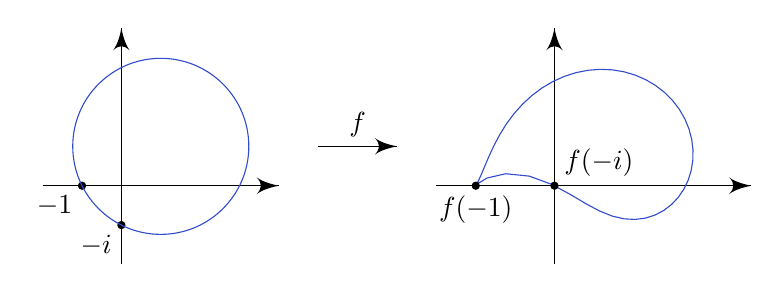
\begin{tikzpicture}[scale=0.5]
      \draw [->] (-2, 0) -- (4, 0);
      \draw [->] (0, -2) -- (0, 4);
      \node [circ] at (-1, 0) {};
      \node [circ] at (0, -1) {};
      \node at (-1, 0) [anchor = north east] {$-1$};
      \node at (0, -1) [anchor = north east] {$-i$};
      \draw [mblue] (1, 1) circle [radius=2.236];

      \draw [->] (5, 1) -- (7, 1) node [pos=0.5, above] {$f$};

      \begin{scope}[shift={(11, 0)}]
        \draw [->] (-3, 0) -- (5, 0);
        \draw [->] (0, -2) -- (0, 4);
        \draw [mblue, domain=0:360, samples=50] plot ({(sqrt (7 + 4.4721*(sin(\x) + cos(\x))) + 1/(sqrt (7 + 4.4721*(sin(\x) + cos(\x))))) * (2.236*cos(\x) + 1)/(sqrt (7 + 4.4721*(sin(\x) + cos(\x))))},{(sqrt (7 + 4.4721*(sin(\x) + cos(\x))) - 1/(sqrt (7 + 4.4721*(sin(\x) + cos(\x))))) * (2.236*sin(\x) + 1)/(sqrt (7 + 4.4721*(sin(\x) + cos(\x))))});
        \node [circ] at (-2, 0) {};
        \node [circ] at (0, 0) {};
        \node at (-2, 0) [below] {$f(-1)$};
        \node at (0, 0) [anchor = south west] {$f(-i)$};
      \end{scope}
    \end{tikzpicture}
  \end{center}
  Note that we have a singularity at $f(-1) = -1$. This is exactly the point where $f$ is not conformal, and is no longer required to preserve angles.

  This is a crude model of an aerofoil, and the transformation is known as the Joukowsky transform.

  In applied mathematics, this is used to model fluid flow over a wing in terms of the analytically simpler flow across a circular section. This is (apparently) useful because the Laplace's equation comes up a lot in fluid flow, and we have seen a connection between Laplace's equation and analytic functions.
\end{eg}

We interlude with a little trick. Often, there is no simple way to describe regions in space. However, if the region is bounded by circular arcs, there is a trick that can be useful.

Suppose we have a circular arc between $\alpha$ and $\beta$.
\begin{center}
  \begin{tikzpicture}
    \draw (0, 0) -- (8 ,0);
    \draw [dashed] (1, 0) -- (4, 2) -- (6, 0);
    \node [circ] (a) at (3, 1.333) {};
    \node [circ] (c) at (5, 1) {};
    \node [circ] (b) at (4, 2) {};
    \node at (a) [left] {$\alpha$};
    \node at (b) [above] {$z$};
    \node at (c) [right] {$\beta$};
    \drawcirculararc(5, 1)(4,2)(3, 1.333);

    \draw (1.4, 0) arc(0:33.69:0.4);
    \node [right] at (1.4, 0.2) {$\phi$};
    \draw (6.4, 0) arc(0:135:0.4);
    \node [right] at (6.4, 0.2) {$\theta$};
    \draw (4.2828, 1.7172) arc(315:213.69:0.4);
    \node [below] at (4, 1.6) {$\mu$};
  \end{tikzpicture}
\end{center}
Along this arc, $\mu = \theta - \phi = \arg(z - \alpha) - \arg(z - \beta)$ is constant. Thus, for each $\mu$, we get an arc from $\alpha$ to $\beta$.

To obtain a region bounded by two arcs, we find the two $\mu_-$ and $\mu_+$ that describe the boundary arcs. Then a point lie between the two arcs if and only if its $\mu$ is in between $\mu_-$ and $\mu_+$, ie. the region is
\[
  \left\{z: \arg\left(\frac{z - \alpha}{z - \beta}\right) \in [\mu_-, \mu_+]\right\}.
\]
This says the point has to lie in some arc between those given by $\mu_-$ and $\mu_+$.

For example, the following region:
\begin{center}
  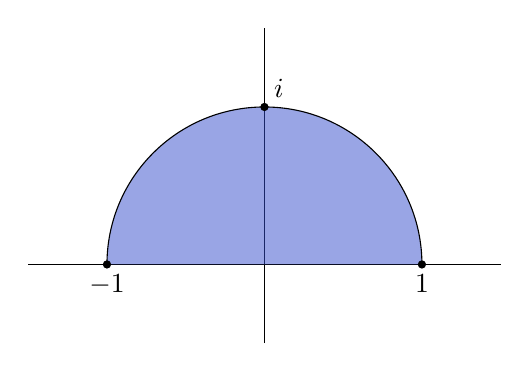
\begin{tikzpicture}
    \draw (-3, 0) -- (3, 0);
    \draw (0, -1) -- (0, 3);
    \fill [mblue, opacity=0.5] (2, 0) arc (0:180:2) -- (2, 0);
    \draw (2, 0) arc (0:180:2);
    \node [circ] at (-2, 0) {};
    \node [circ] at (2, 0) {};
    \node [circ] at (0, 2) {};
    \node at (-2, 0) [below] {$-1$};
    \node at (2, 0) [below] {$1$};
    \node at (0, 2) [anchor = south west] {$i$};
  \end{tikzpicture}
\end{center}
can be given by
\[
  \mathcal{U} = \left\{z: \arg\left(\frac{z - 1}{z + 1}\right) \in \left[\frac{\pi}{2}, \pi\right]\right\}.
\]
Thus for instance the map
\[
  z \mapsto -\left(\frac{z - 1}{z + 1}\right)^2
\]
is a conformal equivalence from $\mathcal{U}$ to $\H$. This is since if $z \in \mathcal{U}$, then $\frac{z - 1}{z + 1}$ has argument in $\left[\frac{\pi}{2}, \pi\right]$. Squaring doubles the angle and gives the lower half-plane, and multiplying by $-1$ gives the upper half plane.
\begin{center}
  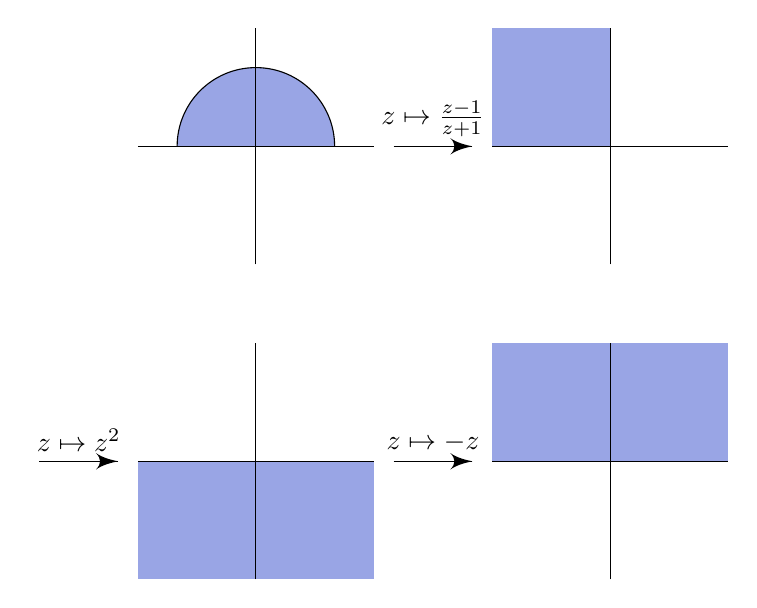
\begin{tikzpicture}[scale=0.5]
    \fill [mblue, opacity=0.5] (2, 0) arc (0:180:2) -- (2, 0);
    \draw (2, 0) arc (0:180:2);
    \draw (-3, 0) -- (3, 0);
    \draw (0, -3) -- (0, 3);

    \draw [->] (3.5, 0) -- (5.5, 0) node [pos=0.5, above] {$z \mapsto \frac{z - 1}{z + 1}$};
    \begin{scope}[shift={(9,0)}]
      \fill [mblue, opacity=0.5] (-3, 3) rectangle (0, 0);
      \draw (-3, 0) -- (3, 0);
      \draw (0, -3) -- (0, 3);

    \end{scope}
    \begin{scope}[shift={(0,-8)}]
      \draw [->] (-5.5, 0) -- (-3.5, 0) node [pos=0.5, above] {$z \mapsto z^2$};

      \fill [mblue, opacity=0.5] (-3, 0) rectangle (3, -3);
      \draw (-3, 0) -- (3, 0);
      \draw (0, -3) -- (0, 3);

      \draw [->] (3.5, 0) -- (5.5, 0) node [pos=0.5, above] {$z \mapsto -z$};
    \end{scope}
    \begin{scope}[shift={(9,-8)}]
      \fill [mblue, opacity=0.5] (-3, 0) rectangle (3, 3);
      \draw (-3, 0) -- (3, 0);
      \draw (0, -3) -- (0, 3);
    \end{scope}
  \end{tikzpicture}
\end{center}
In fact, there is a really powerful theorem telling us most things are conformally equivalent to the unit disk.

\begin{thm}[Riemann mapping theorem]
  Let $\mathcal{U} \subseteq \C$ be the bounded domain enclosed by a simple closed curve, or more generally any simply connected domain not equal to all of $\C$. Then $\mathcal{U}$ is conformally equivalent to $D = \{z: |z| < 1\} \subseteq \C\}$.
\end{thm}
This in particular tells us any two simply connected domains are conformally equivalent.

\begin{defi}[Simple closed curve]
  A \emph{simple closed curve} is the image of an injective map $S^1 \to \C$.
\end{defi}
It should be clear (though not trivial to prove) that a simple closed curve separates $\C$ into a bounded part and an unbounded part.

The more general statement requires the following definition:
\begin{defi}[Simply connected]
  A domain $\mathcal{U}\subseteq \C$ is \emph{simply connected} if every continuous map from the circle $f: S^1 \to \mathcal{U}$ can be extended to a continuous map from the disk $F: \overline{D^2} \to \mathcal{U}$ such that $F|_{\partial \overline{D^2}} = f$. Alternatively, any loop can be continuously shrunk to a point.
\end{defi}

\begin{eg}
  The unit disk is simply-connected, but the region defined by $1 < |z| < 2$ is not, since the circle $|z| = 1.5$ cannot be extended to a map from a disk.
  \begin{center}
    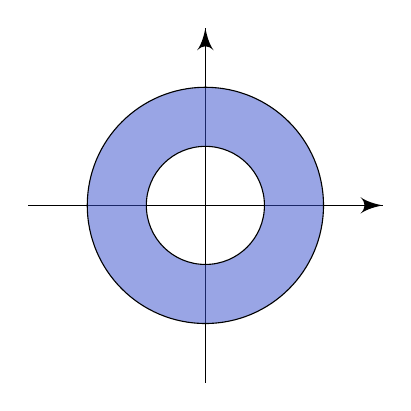
\begin{tikzpicture}[scale=0.75]
      \draw [->] (-3, 0) -- (3, 0);
      \draw [->] (0, -3) -- (0, 3);
      \fill [mblue, opacity=0.5] circle [radius=2];
      \fill [white] circle [radius=1];
      \draw circle [radius=1];
      \draw circle [radius=2];
      \draw (-1, 0) -- (1, 0);
      \draw (0, -1) -- (0, 1);
    \end{tikzpicture}
  \end{center}
\end{eg}
We will not prove this statement, but it is nice to know that this is true.

If we believe that the unit disk is relatively simple, then since all simply connected regions are conformally equivalent to the disk, all simply connected domains are boring. This suggests we will later encounter domains with holes to make the course interesting. This is in fact true, and we will study these holes in depth later.

\begin{eg}
  The exponential function
  \[
    e^z = 1 + z + \frac{z^2}{2!} + \frac{z^3}{3!} + \cdots
  \]
  defines a function $\C \to \C^*$. In fact it is a conformal mapping. This sends the region $\{z: \Re(z) \in [a, b]\}$ to the annulus $\{e^a \leq |w| \leq e^b\}$. One is simply connected, but the other is not --- this is not a problem since $e^z$ is \emph{not} bijective on the strip.
  \begin{center}
    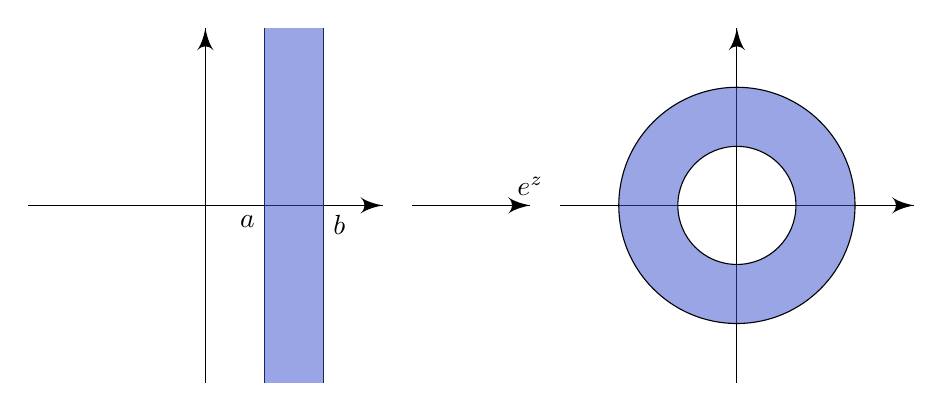
\begin{tikzpicture}[scale=0.75]
      \draw [->] (-3, 0) -- (3, 0);
      \draw [->] (0, -3) -- (0, 3);

      \draw (1, 3) -- (1, -3);
      \draw (2, 3) -- (2, -3);
      \fill [mblue, opacity=0.5] (1, 3) rectangle (2, -3);
      \node [anchor=north east] at (1, 0) {$a$};
      \node [anchor=north west] at (2, 0) {$b$};

      \draw [->] (3.5, 0) -- (5.5, 0) node [above] {$e^z$};
      \begin{scope}[shift={(9, 0)}]
        \draw [->] (-3, 0) -- (3, 0);
        \draw [->] (0, -3) -- (0, 3);
        \fill [mblue, opacity=0.5] circle [radius=2];
        \fill [white] circle [radius=1];
        \draw circle [radius=1];
        \draw circle [radius=2];
        \draw (-1, 0) -- (1, 0);
        \draw (0, -1) -- (0, 1);
      \end{scope}
    \end{tikzpicture}
  \end{center}
\end{eg}

\subsection{Power series and logarithms}
At this point, we need to recall some facts from IB Analysis II.
\begin{defi}[Uniform convergence]
  A sequence $(f_n)$ of functions \emph{converge uniformly} to $f$ if for all $\varepsilon > 0$, there is some $N$ such that $n > N$ implies $|f_n(z) - f(z)| < \varepsilon$ for all $z$.
\end{defi}

\begin{prop}
  The uniform limit of continuous functions is continuous.
\end{prop}

We also had the following nice test for uniform convergence of a series:
\begin{prop}[Weierstrass M-test]
  For a sequence of functions $f_n$, if we can find $(M_n) \subseteq \R_{>0}$ such that $|f_n(x)| < M_n$ for all $x$ in the domain, then $\sum M_n$ converges implies $\sum f_n(x)$ converges uniformly on the domain.
\end{prop}

Finally, we have the following result.
\begin{prop}
  Given any constants $\{c_n\}_{n \geq 0} \subseteq \C$, there is a unique $R \in [0, \infty]$ such that the series $z \mapsto \sum_{n = 0}^\infty c_n(z - a)^n$ converges absolutely if $|z - a| < R$ and diverges if $|z - a| > R$. Moreover, if $0 < r < R$, then the series converges uniformly on $|z| < r$. This $R$ is known as the \emph{radius of convergence}.
\end{prop}
So while we don't necessarily get uniform convergence on the whole domain, we get uniform convergence on all compact subsets of the domain.

We are now going to look at power series. They will serve as examples, and as we will see later, universal examples, of holomorphic functions.

\begin{thm}
  Let
  \[
    f(z) = \sum_{n = 0}^\infty c_n (z - a)^n
  \]
  be a power series with radius of convergence $R > 0$. Then
  \begin{enumerate}
    \item $f$ is holomorphic on $B(a; R) = \{z: |z - a| < R\}$.
    \item $f'(z) = \sum n c_n (z - 1)^{n - 1}$, which also has radius of convergence $R$.
    \item Therefore $f$ is infinitely complex differentiable on $B(a; R)$. Furthermore,
      \[
        c_n = \frac{f^{(n)}(a)}{n!}.
      \]
  \end{enumerate}
\end{thm}

\begin{proof}
  Without loss of generality, take $a = 0$. The third part obviously follows from the previous two, and we will prove the first two parts simultaneously. We would like to first prove that the series has radius of convergence $R$, so that we can freely happily manipulate it.

  Certainly, we have $|n c_n| \geq |c_n|$. So by comparison to the series for $f$, we can see that the radius of convergence of $\sum n c_n z^{n - 1}$ is at most $R$. But if $|z| < \rho < R$, then we can see
  \[
    \frac{|n c_n z^{n - 1}|}{|c_n \rho^{n - 1}|} = n \left|\frac{z}{\rho}\right|^{n - 1} \to 0
  \]
  as $n \to \infty$. So by comparison to $\sum c_n \rho^{n - 1}$, which converges, we see that the radius of convergence of $\sum n c_n z^{n - 1}$ is at least $\rho$. So the radius of convergence must be exactly $R$.

  Now we want to show $f$ really is differentiable with that derivative. Pick $z, w$ such that $|z|, |w| \leq \rho$ for some $\rho < R$ as before.

  Define a new function
  \[
    \varphi (z, w) = \sum_{n = 1}^\infty c_n \sum_{j = 0}^{n - 1} z^j w^{n - 1 - j}.
  \]
  Noting
  \[
    \left|c_n \sum_{j = 0}^{n - 1} z^j w^{n - 1 - j}\right| \leq n |c_n| \rho^n,
  \]
  we know the series defining $\varphi$ converges uniformly on $\{|z| \leq \rho, |w| < \rho\}$, and hence to a continuous limit.

  If $z \not= w$, then using the formula for the (finite) geometric series, we know
  \[
    \varphi(z, w) = \sum_{n = 1}^\infty c_n\left(\frac{z^n - w^n}{z - w}\right) = \frac{f(z) - f(w)}{z - w}.
  \]
  On the other hand, if $z = w$, then
  \[
    \varphi(z, z) = \sum_{n = 1}^\infty c_n n z^{n - 1}.
  \]
  Since $\varphi$ is continuous, we know
  \[
    \lim_{w \to z} \frac{f(z) - f(w)}{z - w} \to \sum_{n = 1}^\infty c_n nz^{n - 1}.
  \]
  So $f'(z) = \varphi(z, z)$ as claimed. Then (iii) follows from (i) and (ii) directly.
\end{proof}

\begin{cor}
  Given a power series
  \[
    f(z) = \sum_{n \geq 0} c_n (z - a)^n
  \]
  with radius of convergence $R > 0$, and given $0 < \varepsilon < R$, if $f$ vanishes on $B(a, \varepsilon)$, then $f$ vanishes identically.
\end{cor}

\begin{proof}
  If $f$ vanishes on $B(a, \varepsilon)$, then all its derivatives vanish, and hence the coefficients all vanish. So it is identically zero.
\end{proof}
This is obviously true, but will come up useful some time later.

It is might be useful to have an explicit expression for $R$. For example, we can have
\begin{align*}
  R &= \sup \{r \geq 0: |c_n|r^n \to 0\text{ as }n \to \infty\}\\
  &= \frac{1}{\limsup \sqrt[n]{|c_n|}}.
\end{align*}
But we probably won't need these.

Recall that the exponential function
\[
  e^z = \exp(z) = 1 + z + \frac{z^2}{2!} + \frac{z^3}{3!} + \cdots
\]
has a radius of convergence of $\infty$. So it is an entire function. We have the usual standard properties, such as $e^{z + w} = e^z e^w$, and also
\[
  e^{x + iy} = e^x e^{iy} = e^x(\cos y + i \sin y).
\]
So given $w \in \C^* = \C\setminus\{0\}$, there are solutions to $e^z = w$. In fact, this has infinitely many solutions, differing by adding integer multiples of $2\pi i$. In particular, $e^z = 1$ if and only if $z$ is an integer multiple of $2\pi i$.

This means we have to be a bit more careful if we want to talk about the inverse function of the exponential. We make the following definition:

\begin{defi}[Branch of logarithm]
  Let $U \subseteq \C^*$ be an open subset. A \emph{branch of the logarithm} on $U$ is a continuous function $\lambda: U \to \C$ for which $e^{\lambda (z)} = z$ for all $z \in U$.
\end{defi}
This is like a ``local inverse'' to the exponential function. These need not exist for all $U$. For example, there is no branch of the logarithm on the whole $\C^*$, as we will later prove.

\begin{eg}
  Let $U = \C\setminus \R_{\leq 0}$, a ``slit plane''.
  \begin{center}
    \begin{tikzpicture}
      \draw [->] (0, 0) -- (2, 0);
      \draw [thick] (-2, 0) -- (0, 0);
      \draw [->] (0, -2) -- (0, 2);
      \node [circ] at (0, 0) {};
    \end{tikzpicture}
  \end{center}
  Then for each $z \in U$, we write $z = r^{i \theta}$, with $-\pi < \theta < \pi$. Then $\lambda(z) = \log (r) + i \theta$ is a branch of the logarithm. This is the \emph{principal branch}.

  On $U$, there is a continuous function $\arg: U \to (-\pi, \pi)$, which is why we can construct a branch. This is not true on, say, the unit circle.
\end{eg}

\begin{prop}
  On $\{z \in \C: z \not\in \R_{\leq 0}\}$, the principal branch $\log: U \to \C$ is holomorphic function. Moreover,
  \[
    \frac{\d}{\d z}\log z = \frac{1}{z}.
  \]
  If $|z| < 1$, then
  \[
    \log (1 + z) = \sum_{n \geq 1} (-1)^{n - 1} \frac{z^n}{n} = z - \frac{z^2}{2} + \frac{z^3}{3} - \cdots.
  \]
\end{prop}

\begin{proof}
  That logarithm is holomorphic follows from the chain rule and $e^{\log z} = z$. This shows $\frac{\d}{\d z} (\log z) = \frac{1}{z}$.

  To show that $\log(1 + z)$ is indeed given by the said power series, note that the power series does have a radius of convergence $1$ by, say, the ratio test. So by the previous result, it has derivative
  \[
    1 - z + z^2 + \cdots = \frac{1}{1 + z}.
  \]
  Therefore, $\log(1 + z)$ and the power series have equal derivative, and hence coincide up to a constant. Since they agree at $z = 0$, they must in fact be equal.
\end{proof}
Note that if $\alpha \in \C$ and $\log: U \to \C$ is a branch of the logarithm, we can define
\[
  z^{\alpha} = e^{\alpha \log z}
\]
on $U$.

We can view $\log$ as a multivalued function on $\C^*$. In general, we say that a point $p \in \C $ is a \emph{branch point} of a multivalued function if the function cannot be given a continuous single-valued definition in a (punctured) neighbourhood $B(p, \varepsilon) \setminus \{p\}$ of $p$ for any $\varepsilon > 0$. For example, $0$ is a branch point of $\log$.

\begin{eg}
  Consider the function
  \[
    f(z) = \sqrt{z(z - 1)}.
  \]
  This has \emph{two} branch points, $z = 0$ and $z = 1$, since we cannot consistently a square root consistently near $0$, as it is defined via the logarithm.
\end{eg}

Note we can define a continuous branch of $f$ on either
\begin{center}
  \begin{tikzpicture}
    \draw [->] (-2, 0) -- (2, 0);
    \draw [thick] (-2, 0) -- (0, 0);
    \draw [thick] (1, 0) -- (2, 0);
    \draw [->] (0, -2) -- (0, 2);
    \node [below] at (1, 0) {$1$};
    \node [anchor = north east] {$0$};
    \node [circ] at (1, 0) {};
    \node [circ] at (0, 0) {};
  \end{tikzpicture}
\end{center}
or we can just kill a finite slit by
\begin{center}
  \begin{tikzpicture}
    \draw [->] (-2, 0) -- (2, 0);
    \draw [thick] (1, 0) -- (0, 0);
    \draw [->] (0, -2) -- (0, 2);
    \node [below] at (1, 0) {$1$};
    \node [anchor = north east] {$0$};
    \node [circ] at (1, 0) {};
    \node [circ] at (0, 0) {};
  \end{tikzpicture}
\end{center}
Why is the second case possible? Note that
\[
  f(z) = e^{\frac{1}{2}(\log(z) + \log(z - 1))}.
\]
If we move around a path encircling the finite slit, the argument of each of $f(z)$ and $\log(z - 1)$ will jump by $2\pi i$, and the total change in the exponent is $2\pi i$. So the expression for $f(z)$ becomes uniquely defined.

While these two ways of cutting slits look rather different, if we consider this to be on the Riemann sphere, then these two cuts now look similar. It's just that one passes through the point $\infty$, and the other doesn't.

However, this is not a very good treatment of the problem. A better treatment will be performed in the IID Riemann Surfaces course.

\section{Contour integration}
Our next task is to develop a theory of integration of $\C$-valued functions along paths and closed contours. At first, this would look just like an obvious generalization of real integration. However, this will suddenly become amazing and get a life of its own when we get to Cauchy's theorem.

Recall that a function $f: [a, b] \to \C$ is Riemann integrable if $\Re(f)$ and $\Im (f)$ are individually, by definition. Also, by definition,
\[
  \int_a^b f(t) \;\d t = \int_a^b \Re(f(t))\;\d t + i \int_a^b \Im(f(t))\;\d t.
\]
Recall also that if $f$ is continuous, then it is integrable. This will apply in most cases we care about in this course. After all, this is not a course on exotic functions.

We start from some less interesting facts, and slowly develop and prove some really amazing results.
\begin{lemma}
  Suppose $f: [a, b] \to \C$ is continuous (and hence integrable). Then
  \[
    \left|\int_a^b f(t)\;\d t\right| \leq (b - a) \sup_t |f(t)|
  \]
  with equality if and only if $f$ is constant.
\end{lemma}

\begin{proof}
  We let
  \[
    \theta = \arg\left(\int_a^b f(t)\;\d t\right),
  \]
  and
  \[
    M = \sup_t |f(T)|.
  \]
  Then we have
  \begin{align*}
    \left|\int_a^b f(t)\;\d t\right| &= \int_a^b e^{-i\theta} f(t)\;\d t\\
    &= \int_a^b \Re(e^{-i\theta} f(t))\;\d t\\
    &\leq (b - a) M,
  \end{align*}
  with equality if and only if $|f(t)| =M$ and $\arg f(t) = \theta$ for all $t$, ie. $f$ is constant.
\end{proof}

\begin{defi}[Simple path]
  A path $\gamma: [a, b] \to \C$ is \emph{simple} if $\gamma(t_1) = \gamma(t_2)$ only if $t_1 = t_2$ or $\{t_1, t_2\} = \{a, b\}$.
\end{defi}
In other words, it either does not intersect itself, or only intersects itself at the end points.

\begin{defi}[Closed path]
  A path $\gamma: [a, b] \to \C$ is \emph{closed} if $\gamma(a) = \gamma(b)$.
\end{defi}

\begin{defi}[Contour]
  A \emph{contour} is a simple closed path which is piecewise $C^1$, ie. piecewise continuously differentiable.
\end{defi}

For example, it can look something like this:
\begin{center}
  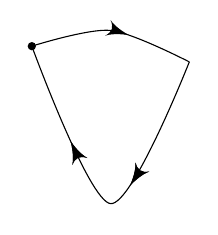
\begin{tikzpicture}[scale=2]
    \draw [->-=0.6] plot [smooth] coordinates {(0, 0) (0.5, 0.1) (1, -0.1)};
    \node [circ] at (0, 0) {};
    \draw [->-=0.4, ->-=0.7] plot [smooth] coordinates {(1, -0.1) (0.5, -1) (0, 0)};
  \end{tikzpicture}
\end{center}

\begin{defi}[Complex integration]
  If $\gamma: [a, b] \to U \subseteq \C$ is $C^1$-smooth and $f: U \to \C$ is continuous, then we define the \emph{integral} of $f$ along $\gamma$ as
  \[
    \int_\gamma f(z) \;\d z = \int_a^b f(\gamma(t)) \gamma'(t) \;\d t.
  \]
  By summing over subdomains, the definition extends to piecewise $C^1$-smooth paths, and in particular contours.
\end{defi}

We have the following properties:
\begin{enumerate}
  \item The definition is insensitive to reparametrization. Let $\phi: [a', b'] \to [a, b]$ be $C^1$ such that $\phi(a') = a, \phi(b') = b$. If $\gamma$ is a $C^1$ path and $\delta= \gamma \circ \phi$, then
    \[
      \int_{\gamma} f(z) \;\d z = \int_{\delta}f(z) \;\d z.
    \]
    This is just the regular change of variables formula, since
    \[
      \int_{a'}^{b'} f(\gamma(\phi(t))) \gamma'(\phi(t)) \phi'(t)\;\d t= \int_a^b f(\gamma(u)) \gamma'(u)\;\d u
    \]
    if $u = \phi(t)$.
  \item If $a < u < b$, then
    \[
      \int_\gamma f(z)\;\d z = \int_{\gamma|_{[a, u]}} f(z)\;\d z + \int_{\gamma|_{[u, b]}}f(z) \;\d z.
    \]
\end{enumerate}
These tells us the integral depends only on the path itself, not how we look at the path or how we cut up the path into pieces.

We also have the following easy properties:
\begin{enumerate}[resume]
  \item If $-\gamma$ is $\gamma$ with reversed orientation, then
    \[
      \int_{-\gamma} f(z)\;\d z = -\int_\gamma f(z)\;\d z.
    \]
  \item If we set for $\gamma: [a, b] \to \C$ the \emph{length}
    \[
      \length(\gamma) = \int_a^b |\gamma'(t)|\;\d t,
    \]
    then
    \[
      \left|\int_\gamma f(z)\;\d z\right| \leq \length (\gamma) \sup_t |f(\gamma(t))|.
    \]
\end{enumerate}

\begin{eg}
  Take $U = \C^*$, and let $f(z) = z^n$ for $n \in \Z$. We pick $\phi: [0, 2\pi] \to U$ that sends $\theta \mapsto e^{i\theta}$. Then
  \[
    \int_\phi f(z)\;\d z =
    \begin{cases}
      2\pi i & n = -1\\
      0& \text{otherwise}
    \end{cases}
  \]
  To show this, we have
  \begin{align*}
    \int_{\phi} f(z)\;\d z &= \int_0^{2\pi} e^{in\theta} ie^{i\theta}\;\d \theta\\
    &= i\int_0^{2\pi} e^{i(n + 1)\theta}\;\d \theta.
  \end{align*}
  If $n = -1$, then the integrand is constantly $1$, and hence gives $2\pi i$. Otherwise, the integrand is a non-trivial exponential which is made of trigonometric functions, and when integrated over $2\pi$ gives zero.
\end{eg}

\begin{eg}
  Take $\gamma$ to be the contour
  \begin{center}
    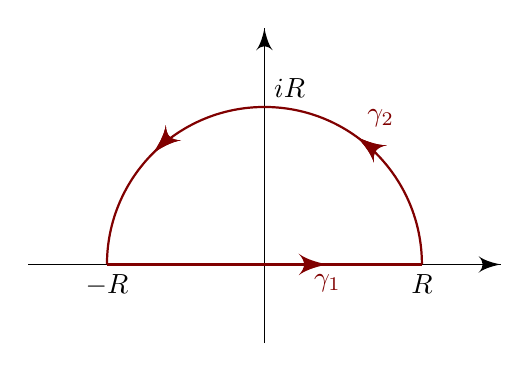
\begin{tikzpicture}
      \draw [->] (-3, 0) -- (3, 0);
      \draw [->] (0, -1) -- (0, 3);
      \draw [thick, mred, ->-=0.7] (-2, 0) -- (2, 0) node [pos=0.7, below] {$\gamma_1$};
      \draw [thick, mred, ->-=0.3, ->-=0.75] (2, 0) arc (0:180:2) node [pos=0.3, anchor = south west] {$\gamma_2$};
      \node [below] at (2, 0) {$R$};
      \node [below] at (-2, 0) {$-R$};
      \node [anchor = south west] at (0, 2) {$iR$};
    \end{tikzpicture}
  \end{center}
  We take the first path to be $\gamma_1: [-R, R] \to \C$ by $\gamma(t) = t$, while $\gamma_2: [0, 1] \to \C$ by $t \mapsto R e^{i\pi t}$.

  Consider the function $f(z) = z^2$. Then the integral is
  \begin{align*}
    \int_\gamma f(z)\;\d z &= \int_{-R}^R t^2 \;\d t + \int_0^1 R^2 e^{2\pi i t} i\pi R e^{i\pi t}\;\d t\\
    &= \frac{2}{3}R^3 + R^3 i\pi \int_0^1 e^{3 \pi i t}\;\d t\\
    &= \frac{2}{3}R^3 + R^3 i\pi \left[\frac{e^{3\pi it}}{3\pi i}\right]_0^1\\
    &= 0
  \end{align*}
\end{eg}
We worked this out explicitly, but this is just an instance of the fundamental theorem of calculus!

\begin{defi}[Antiderivative]
  Let $U \in \C$ and $f: U \to \C$ be continuous. An \emph{antiderivative} of $f$ is a holomorphic function $F: U \to \C$ such that $F'(z) = f(z)$.
\end{defi}

Then the fundamental theorem of calculus tells us:
\begin{thm}[Fundamental theorem of calculus]
  Let $f: U \to \C$ be continuous with antiderivative $F$. If $\gamma: [a, b] \to U$ is piecewise $C^1$-smooth, then
  \[
    \int_\gamma f(z)\;\d z= F(\gamma(b)) - F(\gamma(a)).
  \]
\end{thm}
In particular, the integral depends only on the end points, and not the path itself. Moreover, if $\gamma$ is closed, then the integral vanishes.

\begin{proof}
  We have
  \[
    \int_\gamma f(z)\;\d z = \int_a^b f(\gamma(t)) \gamma'(t) \;\d t = \int_a^b (F \circ \gamma)' (t)\;\d t.
  \]
  Then the result follows from the usual fundamental theorem of calculus, applied to the real and imaginary parts separately.
\end{proof}

\begin{eg}
  This allows us to understand the first example we had. Recall that for $f(z) = z^n$ on $\phi(t) = e^{it}$ (with $0 \leq t \leq 2\pi$), if $n \not= -1$, then
  \[
    f = \frac{\d}{\d t}\left(\frac{z^{n + 1}}{n + 1}\right).
  \]
  So $f$ has a well-defined antiderivative, and the integral vanishes. On the other hand, if $n = -1$, then
  \[
    f(z) = \frac{\d}{\d z} (\log z),
  \]
  where $\log$ can only be defined on a \emph{slit} plane. It is not defined on the whole unit circle. So we cannot apply the fundamental theorem of calculus.

  Reversing the argument around, since $\int_\phi f(z)\;\d z$ does not vanish, this implies there is not a continuous branch of $\log$ on any set $U$ containing the unit circle.
\end{eg}

\begin{prop}
  Let $U \subseteq \C$ be a domain (ie. path-connected non-empty open set), and $f: U \to \C$ be continuous. Moreover, suppose
  \[
    \int_\gamma f(z)\;\d z = 0
  \]
  for any closed piecewise $C^1$-smooth path $\gamma$ in $U$. Then $f$ has an antiderivative.
\end{prop}

This is more-or-less the same proof we gave in IA Vector Calculus that a real function is a gradient if and only if the integral about any closed path vanishes.

\begin{proof}
  Pick our favorite $a_0 \in U$. For $w \in U$, we choose a path $\gamma_w: [0, 1] \to U$ such that $\gamma_w(0) = a_0$ and $\gamma_w(1) = w$. We want to show we can pick $\gamma_w$ such that this is piecewise $C^1$. We already know a \emph{continuous} path $\gamma: [0, 1] \to U$ from $a_0$ to $w$ exists. Since $U$ is open, for all $x$ in the image of $\gamma$, there is some $\varepsilon(x) > 0$ such that $B(x, \varepsilon(x)) \subseteq U$. Since the image of $\gamma$ is compact, it is covered by finitely many such balls. Then it is trivial to pick a piecewise straight path living inside the union of these balls, which is clearly piecewise smooth.

  We thus define
  \[
    F(w) = \int_{\gamma w} f(z)\;\d z.
  \]
  Note that this $F(w)$ is independent of the choice of $\gamma_w$, by our hypothesis on $f$ --- given another choice $\tilde{\gamma}_w$, then $\gamma_w$ concatenated with $-\tilde{\gamma}_w$, written $\gamma_w * (-\tilde{\gamma}_w)$, is a closed piecewise $C^1$ path on $U$. So
  \[
    \int_{\gamma_w * (-\tilde{\gamma}_w)} f(z) \;\d z = 0.
  \]
  The left hand side is
  \[
    \int_{\gamma_W} f(z)\;\d z + \int_{-\tilde{\gamma}_w}f(z)\;\d z = \int_{\gamma_w} f(z)\;\d z - \int_{\tilde{\gamma}_w} f(z) \;\d z.
  \]
  So the two integrals agree.

  Now we need to check that $F$ is complex differentiable. Since $U$ is open, we can pick $\theta > 0$ such that $B(w; \varepsilon) \subseteq U$. Let $\delta_h$ be the radial path in $B(w, \varepsilon)$ from $W$ to $w + h$, with $|h| < \varepsilon$.

  Now note that $\gamma_w * \delta_h$ is a path from $a_0$ to $w + h$. So
  \begin{align*}
    F(w + h) &= \int_{\gamma_w * \delta_h} f(z)\;\d z\\
    &= F(w) + \int_{\delta_h} f(z)\;\d z\\
    &= F(w) + hf(w) + \int_{\delta_h} (f(z) - f(w))\;\d z.
  \end{align*}
  Thus, we know
  \begin{align*}
    \left|\frac{F(w + h) - F(w)}{h} - f(w)\right| &\leq \frac{1}{|h|} \left|\int_{\delta_h} f(z) - f(w)\;\d z\right| \\
    &\leq \frac{1}{|h|} \length(\delta_h) \sup_{\delta_h} |f(z) - f(w)|\\
    &=\sup_{\delta_h} |f(z) - f(w)|.
  \end{align*}
  Since $f$ is continuous, as $h \to 0$, we know $f(z) - f(w) \to 0$. So $F$ is differentiable with derivative $f$.
\end{proof}

In the proof, we constructed the piecewise straight path from $a_0$ to $w$. These paths are nice. In general, we make the following definition:
\begin{defi}[Star-shaped domain]
  A \emph{star-shaped domain} or \emph{star domain} is a domain $U$ such that there is some $p \in U$ such that the line segment $[p, w] \subseteq U$ for all $w \in U$.
  \begin{center}
    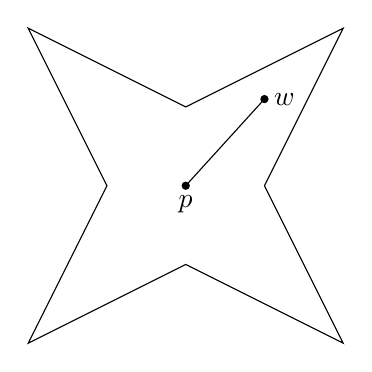
\begin{tikzpicture}
      \draw (1, 0) -- (2, 2) -- (0, 1) -- (-2, 2) -- (-1, 0) -- (-2, -2) -- (0, -1) -- (2, -2) -- (1, 0);
      \node [circ] {};
      \node [below] {$p$};
      \draw (0, 0) -- (1, 1.1) node [circ] {} node [right] {$w$};
    \end{tikzpicture}
  \end{center}
\end{defi}
This is weaker than requiring $U$ to be convex, which says any line segment between \emph{any two points} in $U$, lies in $U$.

Note that we have
\[
  U\text{ is a disc }\Rightarrow U\text{ is convex} \Rightarrow U\text{ is star-shaped} \Rightarrow U\text{ is path-connected},
\]
and none of the implications reverse.

Recall that when constructing the antiderivative, we assumed $\int_\gamma f(z) \;\d z = 0$ for all closed path $\gamma$. We could have required something weaker. All we needed was to intiially pick some $\gamma_w$ for each $w$, and we just need $\int_\gamma f(z)\;\d z = 0$ for all paths of the form $\gamma = \gamma_w * \delta_h * (-\gamma_{w + h})$. If $U$ is a star-shaped domain, then we can pick our pasepoint to be the special point $p$, and then these $\gamma$ are just three straight line segments.

\begin{defi}[Triangle]
  A \emph{triangle} in a domain $U$ is what it ought to be --- the Euclidean convex hull of $3$ points in $U$, lying wholly in $U$. We write its boundary as $\partial T$, which we view as an oriented piecewise $C^1$ path, ie. a contour.
\end{defi}
\begin{center}
  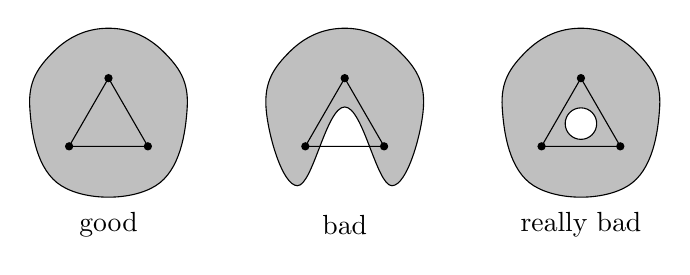
\begin{tikzpicture}
    \begin{scope}[shift={(-3, 0)}]
      \draw [fill=gray!50!white] plot [smooth cycle, tension=0.7] coordinates {(0, 1) (-0.7, 0.7) (-1, 0) (-0.6, -1) (0.6, -1) (1, 0) (0.7, 0.7)};
      \draw (-0.5, -0.5) node [circ] {} -- (0.5, -0.5) node [circ] {} -- (0, 0.366) node [circ] {} -- cycle;

      \node at (0, -1.5) {good};
    \end{scope}

    \begin{scope}
      \draw [fill=gray!50!white] plot [smooth cycle, tension=0.7] coordinates {(0, 1) (-0.7, 0.7) (-1, 0) (-0.6, -1) (0, 0) (0.6, -1) (1, 0) (0.7, 0.7)};
      \draw (-0.5, -0.5) node [circ] {} -- (0.5, -0.5) node [circ] {} -- (0, 0.366) node [circ] {} -- cycle;

      \node at (0, -1.5) {bad};
    \end{scope}

    \begin{scope}[shift={(3, 0)}]
      \draw [fill=gray!50!white] plot [smooth cycle, tension=0.7] coordinates {(0, 1) (-0.7, 0.7) (-1, 0) (-0.6, -1) (0.6, -1) (1, 0) (0.7, 0.7)};
      \draw (-0.5, -0.5) node [circ] {} -- (0.5, -0.5) node [circ] {} -- (0, 0.366) node [circ] {} -- cycle;
      \draw [fill=white] (0, -0.2113) circle [radius=0.2];

      \node at (0, -1.5) {really bad};
    \end{scope}
  \end{tikzpicture}
\end{center}
Our earlier result on constructing antiderivative shows:
\begin{prop}
  If $U$ is a star domain, and $f: U \to \C$ is continuous, and if
  \[
    \int_{\partial T} f(z)\;\d z = 0
  \]
  for all triangles $T \subseteq U$, then $f$ has an antiderivative on $U$.
\end{prop}

\begin{proof}
  As before, taking $\gamma_w = [a_0, w] \subseteq U$ if $U$ is star-shaped about $a_0$.
\end{proof}

This is in some sense a weaker proposition --- while our hypothesis only requires the integral to vanish over triangles, and not arbitrary closed loops, we are restricted to star domains only.

It turns out triangles are in general nice:
\begin{thm}[Cauchy's theorem for a triangle]
  Let $U$ be a domain, and let $f: U \to \C$ be holomorphic. If $T \subseteq U$ is a triangle, then $\int_{\partial T} f(z)\;\d z = 0$.
\end{thm}
So for holomorphic functions, the hypothesis of the previous theorem automatiaclly holds.

We immediately get the following corollary, which is what we will end up using most of the time.
\begin{cor}[Convex Cauchy]
  If $U$ is a convex or star-shaped domain, and $f: U \to \C$ is holomorphic, then for \emph{any} closed piecewise $C^1$ paths $\gamma \in U$, we must have
  \[
    \int_\gamma f(z)\;\d z = 0.
  \]
\end{cor}

\begin{proof}(of corollary)
  If $f$ is holomorphic, then Cauchy's theorem says the integral over any triangle vanishes. If $U$ is star shaped, our proposition says $f$ has an antiderivative. Then the fundamental theorem of calculus tells us the integral around any closed path vanishes.
\end{proof}

Hence, all we need to do is to prove that fact about triangles.
\begin{proof}(of Cauchy's theorem for a triangle)
  Fix a triangle $T$. Let
  \[
    \eta = \left|\int_{\partial T} f(z)\;\d z\right|, \ell = \length (\partial T).
  \]
  The idea is to show for any $\varepsilon > 0$ that $\eta < \varepsilon$, and hence we must have $\varepsilon = 0$. To do so, we subdivide our triangles.

  Before we start, it helps to motivate the idea of subdividing a bit. By subdividing the triangle further and further, we are focusing on a smaller and smaller region of the complex plane. This allows us to study how the integral behaves locally. This is helpful since we are given that $f$ is holomorphic, and holomorphicity is a local property.

  We start with $T = T^0:$
  \begin{center}
    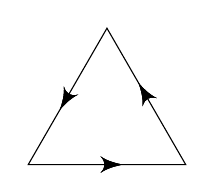
\begin{tikzpicture}
      \draw [->-=0.2, ->-=0.533, ->-=0.866] (0, 0) -- (2, 0) -- (1, 1.732) -- cycle;
    \end{tikzpicture}
  \end{center}
  We then add more lines to get $T_a^0, T_b^0, T_c^0, T_d^0$ (it doesn't really matter which is which).
  \begin{center}
    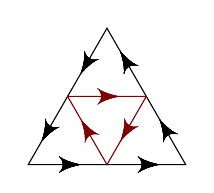
\begin{tikzpicture}
      \draw [->-=0.112, ->-=0.279, ->-=0.445, ->-=0.612, ->-=0.779, ->-=0.945] (0, 0) -- (2, 0) -- (1, 1.732) -- cycle;
      \draw [mred, ->-=0.22, ->-=0.553, ->-=0.886] (1, 0) -- (0.5, 0.866) -- (1.5, 0.866) -- cycle;
    \end{tikzpicture}
  \end{center}
  Then we have
  \[
    \int_{\partial T^0} f(z)\;\d z = \sum_{a, b, c, d} \int_{\partial T^0_{\Cdot}} f(z)\;\d z,
  \]
  if we orient the middle triangle by the anticlockwise orientation, as then each internal edge occurs twice, with opposite orientation.

  For this to be possible, if $\eta = \left|\int_{\partial T^0} f(z)\;\d z\right|$, then there must be some subscript in $\{a, b, c, d\}$ such that
  \[
    \left|\int_{\partial T^0_{\Cdot}} f(z)\;\d z\right| \geq \frac{\eta}{4}.
  \]
  We call this $T_{\Cdot}^0 = T^1$. Then the length of $\partial T^1$ has length
  \[
    \length(\partial T^0_{\Cdot}) = \frac{\ell}{2}.
  \]
  Iterating this, we obtain triangles
  \[
    T^0 \supseteq T^1 \supseteq T^2 \supseteq \cdots
  \]
  such that
  \[
    \left|\int_{\partial T^i} f(z)\;\d z\right| \geq \frac{\eta}{4^i},\quad \length (\partial T^i) = \frac{\ell}{2^i}.
  \]
  Now we are given a nested sequence of closed sets. By IB Metric and Topological Spaces (or IB Analysis II), there is some $z_0 \in \bigcap_{i \geq 0} T^i$.

  Now fix an $\varepsilon > 0$. Since $f$ is holomorphic at $z_0$, we can find a $\delta > 0$ such that
  \[
    |f(w) - f(z_0) - (w - z_0) f'(z_0)| \leq \varepsilon|w - z_0|
  \]
  whenever $|w - z_0| < \delta$. Since the diameters of the triangles are shrinking each time, we can pick an $n$ such that $T^n \subseteq B(z_0, \varepsilon)$. We're almost there. We just need to do one last thing that is slightly sneaky. Note that
  \[
    \int_{\partial T^n} 1 \;\d z = 0 = \int_{\partial T^n} z \;\d z,
  \]
  since these functions certainly do have antiderivatives on $T^n$. Therefore, noting that $f(z_0)$ and $f'(z_0)$ are just constants, we have
  \begin{align*}
    \left|\int_{\partial T^n}f(z)\;\d z\right| &= \left|\int_{\partial T^n} (f(z) - f(z_0) - (z - z_0) f'(z_0))\;\d z\right|\\
    &\leq \int_{\partial T^n} |f(z) - f(z_0) - (z - z_0) f'(z_0)|\;\d z\\
    &\leq \length(\partial T^n) \varepsilon \sup_{z \in \partial T^n}|z - z_0|\\
    &\leq \varepsilon \length(\partial T^n)^2,
  \end{align*}
  since $z_0 \in T^n$, and the distance between any two points in the triangle cannot be greater than the perimeter of the triangle. Substituting our fomulas for these in, we have
  \[
    \frac{\eta}{4^n}\leq \frac{1}{4^n} \ell^2 \varepsilon.
  \]
  So
  \[
    \eta \leq \ell^2 \varepsilon.
  \]
  Since $\ell$ is fixed and $\varepsilon$ was arbitrary, it follows that we must have $\eta = 0$.
\end{proof}
Is this the best we can do? Can we formulate this for an arbitrary domain, and not just star-shaped ones? It is obviously not true if the domain is not simply connected, eg. for $f(z) = \frac{1}{z}$ defined on $\C \setminus \{0\}$. However, it turns out Cauchy's theorem holds as long as the domain is simply connected, but we probably won't get to prove that. However, this is not surprising given the Riemann mapping theorem, since any simply connected domain is conformally eequivalent to the unit disk.

We can generalize our result when $f: U \to \C$ is continuous on the whole of $U$, and holomorphic except on finitely many points. In this case, the same conclusion holds --- $\int_\gamma f(z)\;\d z = 0$ for all piecewise smooth closed $\gamma$.

Why is this? In the proof, it was sufficient to focus on showing $\int_{\partial T} f(z)\;\d z = 0$ for a triangle $T \subseteq U$. Consider the simple case where we only have a single point of non-holomorphicity $a \in T$. The idea is again to subdivide.
\begin{center}
  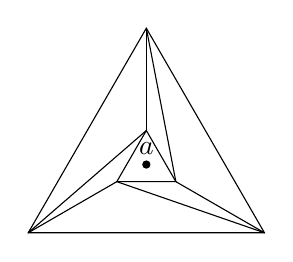
\begin{tikzpicture}[scale=0.75]
    \draw (-2, 0) -- (2, 0) -- (0, 3.464) -- cycle;
    \draw (-0.5, 0.866) -- (0.5, 0.866) -- (0, 1.732) -- cycle;
    \node [circ] at (0, 1.15589) {};
    \node [above] at (0, 1.15589) {$a$};

    \draw (-2, 0) -- (-0.5, 0.866);
    \draw (2, 0) -- (0.5, 0.866);
    \draw (0, 3.464) -- (0, 1.732);

    \draw (-2, 0) -- (0, 1.732);
    \draw (2, 0) -- (-0.5, 0.866);
    \draw (0, 3.464) -- (0.5, 0.866);
  \end{tikzpicture}
\end{center}
We call the center triangle $T'$. Along all other triangles in our subdivision, we get $\int f(z)\;\d z = 0$, as these triangles lie in a region where $f$ is holomorphic. So
\[
  \int_{\partial T} f(z)\;\d z = \int_{\partial T'} f(z)\;\d z.
\]
Note now that we can make $T'$ as small as we like. But
\[
  \left|\int_{\partial T'} f(z)\;\d z\right| \leq \length(\partial T') \sup_{z \in \partial T'} |f(z)|.
\]
Since $f$ is continuous, it is bounded. As we take smaller and smaller subdivisions, $\length(\partial T') \to 0$. So we must have $\int_{\partial T} f(z)\;\d z = 0$.

From here, it's straightforward to conclude the general case --- we can divide the triangle in a way such that each small triangle contains one bad point.

\subsection{The Cauchy integral formula}
We will use that to prove the Cauchy integral formula.

\begin{thm}[Cauchy integral formula]
  Let $U$ be a domain, and $f: U \to \C$ be holomorphic. Suppose there is some $\overline{B(z_0; r)} \subseteq U$ for some $z_0$ and $r > 0$. Then for all $z \in B(z_0; r)$, we have
  \[
    f(z) = \frac{1}{2\pi i} \int_{\partial \overline{B(z_0; r)}} \frac{f(w)}{w - z}\;\d w.
  \]
\end{thm}
Recall that we previously computed $\int_{\partial \overline{B(0, 1)}} \frac{1}{z} \;\d z= 2\pi i$. This is indeed a special case of the Cauchy integral formula. We will provide two proofs. The first proof relies on the above generalization of Cauchy's theorem.

\begin{proof}
  Since $U$ is open, there is some $\delta > 0$ such that $\overline{B(z_0; r + \delta)} \subseteq U$. We define $g: B(z_0; r+ \delta) \to \C$ by
  \[
    g(w) =
    \begin{cases}
      \frac{f(w) - f(z)}{w - z} & w = z\\
      f'(z) & w = z
    \end{cases},
  \]
  where we have \emph{fixed} $z \in B(z_0; r)$ as in the statement of the theorem. Now note that $g$ is holomorphic as a function of $w \in B(z_0, r + \delta)$, except perhaps at $w = z$. But since $f$ is holomorphic, by definition $g$ is continuous everywhere on $B(z_0, r + \delta)$. So the previous result says
  \[
    \int_{\partial \overline{B(z_0; r)}} g(w)\;\d w = 0.
  \]
  This is exactly saying that
  \[
    \int_{\partial \overline{B(z_0; r)}} \frac{f(w)}{w - z} = \int_{\partial \overline{B(z_0; r)}} \frac{f(z)}{w - z}\;\d w.
  \]
  We now rewrite
  \[
    \frac{1}{w - z} = \frac{1}{w - z_0} \cdot \frac{1}{1 - \left(\frac{z - z_0}{w - z_0}\right)} = \sum_{n = 0}^\infty \frac{(z - z_0)^n}{(w - z_0)^{n + 1}}.
  \]
  Note that this sum converges uniformly on $\partial \overline{B(z_0; r)}$ since
  \[
    \left|\frac{z - z_0}{w - z_0}\right| < 1
  \]
  for $w$ on this circle.

  By uniform convergence, we can exchange summation and integration. So
  \[
    \int_{\partial \overline{B(z_0; r)}} \frac{f(w)}{w - z} \;\d w = \sum_{n = 0}^\infty \int_{\partial \overline{B(z_0, r)}} f(z) \frac{(z - z_0)^n}{(w - z_0)^{n + 1}}\;\d w.
  \]
  We note that $f(z) (z - z_0)^n$ is just a constant, and that we have previously proven
  \[
    \int_{\partial \overline{B(z_0; r)}} (w - z_0)^k \;\d w =
    \begin{cases}
      2\pi i & k = -1\\
      0 & k \not= -1
    \end{cases}.
  \]
  So the right hand side is just $2\pi i f(z)$. So done.
\end{proof}

\begin{cor}[Local maximum principle]
  Let $f: B(z, r) \to \C$ be holomorphic. Suppose $|f(w)| \leq |f(z)|$ for all $w \in B(z; r)$. Then $f$ is constant. In other words, a non-constant function cannot achieve an interior local maximum.
\end{cor}

\begin{proof}
  Let $0 < \rho < r$. Applying the Cauchy integral formula, we get
  \begin{align*}
    |f(z)| &= \left|\frac{1}{2\pi i}\int_{\partial \overline{B(z; \rho)}} \frac{f(w)}{w - z}\;\d w\right|\\
    \intertext{Setting $w = z + \rho e^{2\pi i\theta}$, we get}
    &= \left|\int_0^1 f(z + \rho e^{2 \pi i \theta})\;\d \theta\right|\\
    &\leq \sup_{|z - w| = \rho} |f(w)|\\
    &\leq f(z).
  \end{align*}
  So we must have equality throughout. When we proved the supremum bound for the integral, we showed equality can happen only if the integrand is constant. So $|f(w)|$ is constant on the circle $|z - w| = \rho$, and is equal to $f(z)$. Since this is true for all $\rho \in (0, r)$, it follows that $|f|$ is constant on $B(z; r)$. Then the Cauchy-Riemann equations then entail that $f$ must be constant, as you have shown in example sheet 1.
\end{proof}
In particular, since harmonic functions in $\R^2$ are the real parts of holomorphic functions, the same result holds for harmonic functions as well, as we have seen in IA Vector Calculus, via a similar argument.

Going back to the Cauchy integral formula, recall that we had $\overline{B(z_0; r)} \subseteq U$, $f: U \to C$ holomorphic, and we want to show
\[
  f(z) = \frac{1}{2\pi i} \int_{\partial \overline{B(z_0; r)}} \frac{f(w)}{w - z}\;\d w.
\]
When we proved it last time, we remember we know how to integrate things of the form $\frac{1}{(w - z_0)^n}$, and manipulated the formula such that we get the integral is made of things like this.

The second strategy is to change the contour of integration instead of changing the integrand. If we can change it so that the integral is performed over a circle around $z$ instead of $z_0$, then we know what to do.
\begin{center}
  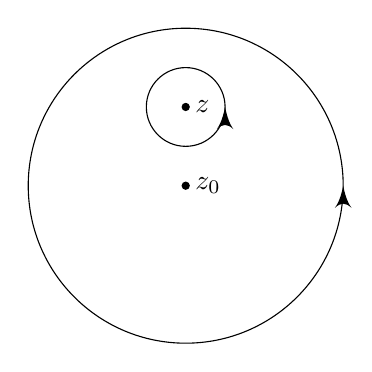
\begin{tikzpicture}
    \node [circ] {};
    \node [right] {$z_0$};
    \draw [->] circle [radius=2]; % arrow counterclockwise

    \node [circ] at (0, 1) {};
    \node [right] at (0, 1) {$z$};
    \draw [->] (0, 1) circle [radius=0.5];
  \end{tikzpicture}
\end{center}
\begin{proof}(of Cauchy integral formula again)
  Given $\varepsilon > 0$, we pick $\delta > 0$ such that $\overline{B(z, \delta)} \subseteq B(z_0, r)$, and such that whenever $|w - z| + \delta$, then $|f(w) - f(z)| < \varepsilon$. This is possible since $f$ is uniformly continuous on the neighbourhood of $z$. We now cut our region apart:
  \begin{center}
    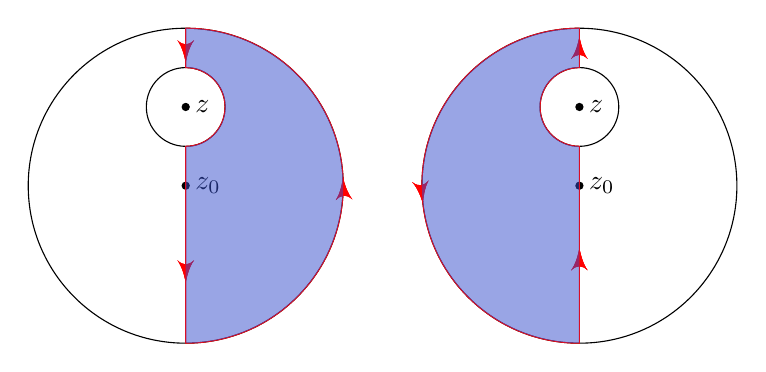
\begin{tikzpicture}
      \node [circ] {};
      \node [right] {$z_0$};
      \draw circle [radius=2];

      \node [circ] at (0, 1) {};
      \node [right] at (0, 1) {$z$};
      \draw (0, 1) circle [radius=0.5];

      \draw [red, ->-=0.04, ->-=0.35, ->-=0.72] (0, 2) -- (0, 1.5) arc(90:-90:0.5) -- (0, -2) arc(-90:90:2);
      \fill [mblue, opacity=0.5] (0, 2) -- (0, 1.5) arc(90:-90:0.5) -- (0, -2) arc(-90:90:2);

      \begin{scope}[shift={(5, 0)}]
        \node [circ] {};
        \node [right] {$z_0$};
        \draw circle [radius=2];

        \node [circ] at (0, 1) {};
        \node [right] at (0, 1) {$z$};
        \draw (0, 1) circle [radius=0.5];

        \draw [red, -<-=0.01, -<-=0.31, -<-=0.69] (0, 2) -- (0, 1.5) arc(90:270:0.5) -- (0, -2) arc(270:90:2);
        \fill [mblue, opacity=0.5] (0, 2) -- (0, 1.5) arc(90:270:0.5) -- (0, -2) arc(270:90:2);
      \end{scope}
    \end{tikzpicture}
  \end{center}
  We know $\frac{f(w)}{w - z}$ is holomorphic on sufficiently small open neighbourhoods of the half-contours indicated. The area enclosed by the contours might not be star-shaped, but we can definitely divide it once more so that it is. Hence the integral of $\frac{f(w)}{w - z}$ around the half-contour vanishes by Cauchy's theorem. Adding these together, we get
  \[
    \int_{\partial \overline{B(z_0, r)}} \frac{f(w)}{w - z}\;\d w = \int_{\partial \overline{B(z, \delta)}} \frac{f(w)}{w - z}\;\d w,
  \]
  where the balls are both oriented anticlockwise. now we have
  \[
    \left|f(z) - \frac{1}{2\pi i} \int_{\partial \overline{B(z_0, r)}} \frac{f(w)}{w - z}\;\d w\right| = \left|f(z) - \frac{1}{2\pi i} \int_{\partial \overline{B(z, \delta)}} \frac{f(w)}{w - z}\;\d w\right|.
  \]
  Now we once again use the fact that
  \[
    \int_{\partial \overline{B(z, \delta)}} \frac{1}{w - z}\;\d z = 2\pi i
  \]
  to show this is equal to
  \[
    \left|\frac{1}{2\pi i} \int_{\partial \overline{B(z, \delta)}} \frac{f(z) - f(w)}{w - z} \;\d w\right| \leq \frac{1}{2\pi} \cdot 2\pi \delta \cdot \frac{1}{\delta} \cdot \varepsilon = \varepsilon.
  \]
  Taking $\varepsilon \to 0$, we see that the Cauchy integral formula holds.
\end{proof}
Note that the subdivision we did above was something we can do in general.

\begin{defi}[Elementary deformation]
  Given a pair of $C^1$-smooth (or piecewise smooth) closed paths $\phi, \psi: [0, 1] \to U$, we say $\psi$ is an elementary deformation of $\phi$ if there exists convex open sets $C_1, \cdots, C_n \subseteq U$ and a division of the interval $0 = x_0 < x_1 < \cdots < x_n = 1$ such that on $[x_{i - 1}, x_i]$, both $\phi(t)$ and $\psi(t)$ both belong to $C_i$.
\end{defi}
\begin{center}
  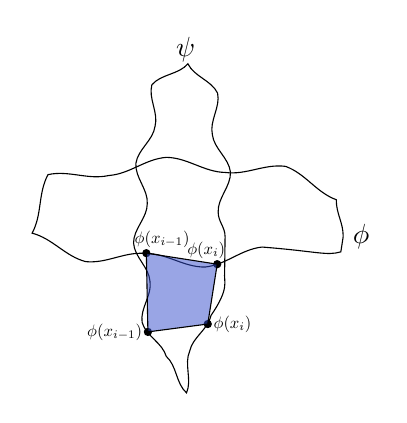
\begin{tikzpicture}
    \draw [decorate, decoration={snake, segment length=1.5cm}] ellipse (2 and 0.5);
    \node [right] at (2, 0) {$\phi$};
    \draw [decorate, decoration={snake, segment length=1cm}] ellipse (0.5 and 2);
    \node [above] at (0, 2.1) {$\psi$};;

    \node [circ] at (-0.5, -0.21) {};
    \node [scale=0.6, above] at (-0.3, -0.21) {$\phi(x_{i - 1})$};

    \node [circ] at (0.4, -0.35) {};
    \node [scale=0.6, above] at (0.26, -0.35) {$\phi(x_i)$};

    \node [circ] at (-0.48, -1.21) {};
    \node [scale=0.6, left] at (-0.48, -1.21) {$\phi(x_{i - 1})$};

    \node [circ] at (0.28, -1.11) {};
    \node [scale=0.6, right] at (0.28, -1.11) {$\phi(x_i)$};

    \draw [fill opacity=0.5, fill=mblue] (-0.5, -0.21) -- (0.4, -0.35) -- (0.28, -1.11) -- (-0.48, -1.21) -- cycle;
  \end{tikzpicture}
\end{center}
Then there are straight lines $\gamma_i: \phi(x_i) \to \psi(x_i)$ lying inside $C_i$. If $f$ is holomorphic on $U$, considering the shaded square, we find
\[
  \int_\phi f(z)\;\d z = \int_\psi f(z)\;\d z
\]
when $\phi$ and $\psi$ are convex deformations.

We now explore some classical consequences of the Cauchy Integral formula.
\subsection{Liouville's theorem}
\begin{thm}[Liouville's theorem]
  Let $f: \C \to \C$ be an entire function (ie. holomorphic everywhere). If $f$ is bounded, then $f$ is constant.
\end{thm}
This, for example, means there is no interesting holomorphic period functions like $\sin$ and $\cos$ that are bounded everywhere.

\begin{proof}
  Suppose $|f(z)| \leq M$ for all $z \in \C$. We fix $z_1, z_2 \in \C$, and estimate $|f(z_1) - f(z_2)|$ with the integral formula.

  Let $R > \max \{2 |z_1|, 2|z_2|\}$. By the integral formula, we know
  \begin{align*}
    |f(z_1) - f(z_2)| &= \left|\frac{1}{2\pi i}\int_{\partial B(0, R)} \left(\frac{f(w)}{w - z_1} - \frac{f(w)}{w - z_2}\right)\;\d w\right|\\
    &= \left|\frac{1}{2\pi i}\int_{\partial B(0, R)} \frac{f(w)(z_1 - z_2)}{(w - z_1)(w - z_2)} \;\d w\right|\\
    &\leq \frac{1}{2\pi} \cdot 2\pi R \cdot \frac{M |z_1 - z_2|}{(R/2)^2} \\
    &= \frac{4M|z_1 - z_2|}{R}.
  \end{align*}
  Note that we get the bound on the denominator since $|w| = R$ implies $|w - z_i| > \frac{R}{2}$ by our choice of $R$. Letting $R \to \infty$, we know we must have $f(z_1) = f(z_2)$. So $f$ is constant.
\end{proof}

\begin{cor}[Fundamental theorem of algebra]
  A non-constant complex polynomial has a root in $\C$.
\end{cor}

\begin{proof}
  Let
  \[
    P(z) = a_n z^n + a_{n - 1}z^{n - 1} + \cdots + a_0,
  \]
  where $a_n \not= 0$ and $n > 0$. So $P$ is non-constant. Thus, as $|z| \to \infty$, $|P(z)| \to \infty$. In particular, there is some $R$ such that for $|z| > R$, we have $|P(z)| \geq 1$.

  Now suppose for contradiction that $P$ does not have a root in $\C$. Then consider
  \[
    f(z) = \frac{1}{P(z)},
  \]
  which is then an entire function, since it is a rational function. On $\overline{B(0, R)}$, we know $f$ is certainly continuous, and hence bounded. Outside this ball, we get $|f(z)| \leq 1$. So $f(z)$ is constant, by Liouville's theorem. But $P$ is non-constant. This is absurd. Hence the result follows.
\end{proof}
Note that there are many many ways we can prove the fundamental theorem of algebra. However, none of them belong wholely to algebra. They all involve some analysis or topology, as you might encounter in the IID Algebraic Topology and IID Riemann Surface courses.

This is not surprising since the construction of $\R$, and hence $\C$, is intrinsically analytic --- we get from $\N$ to $\Z$ by requiring it to have additive inverses; $\Z$ to $\Q$ by requiring multiplicative inverses; $\R$ to $\C$ by requiring the root to $x^2 + 1 = 0$. These are all algebraic. However, to get from $\Q$ to $\R$, we are requiring something about convergence in $\Q$. This is not algebraic. It requires a particular of metric on $\Q$. If we pick a different metric, then you get a different completion, as you may have seen in IB Metric and Topological Spaces. Hence the construction of $\R$ is actually analytic, and not purely algebraic.

\subsection{Taylor's theorem}
Recall our first source of interesting holomorphic came from power series, within their radius of convergence. It turns out these are everything we've got.
\begin{thm}[Taylor's theorem]
  Let $f: B(a, r) \to \C$ be holomorphic. then $f$ has a convergent power series representation
  \[
    f(z) = \sum_{n = 0}^\infty c_n (z - a)^n
  \]
  on $B(a, r)$. Moreover,
  \[
    c_n = \frac{f^{(n)}(a)}{n!} = \frac{1}{2\pi i}\int_{\partial B(a, \rho)}\frac{f(z)}{(z - a)^{n + 1}}\;\d z
  \]
  for any $0 < \rho < r$.
\end{thm}
Note that the very statement of the theorem already implies any holomorphic function has to be infinitely differentiable.
\begin{proof}
  We'll use Cauchy's integral formula. If $|w - a|< \rho < r$, then
  \[
    f(w) = \frac{1}{2\pi i} \int_{\partial B(a, \rho)} \frac{f(z)}{z - w}\;\d z.
  \]
  Now (cf. the first proof of the Cauchy integral formula), we note that
  \[
    \frac{1}{z - w} = \dfrac{1}{(z - a)\left(1 - \frac{w - a}{z - a}\right)} = \sum_{n = 0}^n \frac{(w - a)^n}{(z - a)^{n + 1}}.
  \]
  This series is uniformly convergent everywhere on the $\rho$ disk, including its boundary. By uniform convergence, we can exchange integration and summation to get
  \begin{align*}
    f(w) &= \sum_{n = 0}^\infty \left(\frac{1}{2\pi i} \int_{\partial B(a, \rho)} \frac{f(z)}{(z - a)^{n + 1}}\;\d z\right) (w - a)^n\\
    &= \sum_{n = 0^\infty} c_n (w - a)^n.
  \end{align*}
  Since $c_n$ does not depend on $w$, this is a genuine power series representation, and this is valid on any disk $B(a, \rho) \subseteq B(a, r)$.

  Then the formula for $c_n$ in terms of the derivative comes for free since that's the formula for the derivative of a power series.
\end{proof}
Contrast this with functions like $e^{-1/x^2}$ on $\R$ that have a trivial Taylor series expansion but is non-trivial. This also means we cannot use functions like these to build bump functions that are non-zero only on a compact set (even though we already know this from Liouville's theorem).

\begin{cor}
  If $f: B(a, r) \to \C$ is holomorphic on a disc, then $f$ is infinitely differentiable on the disc.
\end{cor}

\begin{proof}
  Complex power series are infinitely differentiable (and $f$ had better be infinitely differentiable for us to write down the formula for $c_n$ in terms of $f^{(n)}$).
\end{proof}

This justifies our claim from the very beginning that $\Re(f)$ and $\Im(f)$ are harmonic functions if $f$ is holomorphic.

\begin{cor}
  If $f: U\to \C$ is a complex-valued function, then $f = u + iv$ is holomorphic at $p \in U$ if and only if $u, v$ satisfy the Cauchy-Riemann equations, and that $u_x, u_y, v_x, v_y$ are continuous in a neighbourhood of $p$.
\end{cor}

\begin{proof}
  If $u_x, u_y, v_x, v_y$ exist and are continuous in an open neighbourhood of $p$, then $u$ and $v$ are differentiable as functions $\R^2 \to \R^2$ at $p$, and then we proved that the Cauchy-Riemann equations imply differentiability at each point in the neighbourhood of $p$. So $f$ is differentiable at a neighbourhood of $p$.

  On the other hand, if $f$ is holomorphic, then it is infinitely differentiable. In particular, $f'(z)$ is also holomorphic. So $u_x, u_y, v_x, v_y$ are differentiable, hence continuous.
\end{proof}

We also get the following (partial) converse to Cauchy's theorem.
\begin{cor}[Morera's theorem]
  Let $U\subseteq \C$ be a domain. Let $f:U \to \C$ be continuous such that
  \[
    \int_\gamma f(z)\;\d z = 0
  \]
  for all piecewise-$C^1$ closed curves $\gamma \in U$. Then $f$ is holomorphic on $U$.
\end{cor}

\begin{proof}
  We have previously shown that the condition implies that $f$ has an antiderivative $F: U \to \C$, ie. $F$ is a holomorphic function such that $F' = f$. But $F$ is infinitely differentiable. So $f$ must be holomorphic.
\end{proof}

Recall that Cauchy's theorem required $U$ to be sufficiently nice, eg. being star-shaped or just simply-connected. However, Morera's theorem does not. It just requires that $U$ is a domain. This is since holomorphicity is a local property, while vanishing on closed curves is a global result. Cauchy's theorem gets us from a local property to a global property, and hence we need to assume more about what the ``globe'' looks like. On the other hand, passing from a global property to a local one does not. Hence we have this asymmetry.

\begin{cor}
  Let $U \subseteq \C$ be a domain, $f_n; U \to \C$ be a holomorphic function. If $f_n \to f$ uniformly, then $f$ is in fact holomorphic, and
  \[
    f'(z) = \lim_n f_n'(z).
  \]
\end{cor}
\begin{proof}
  Given a piecewise $C^1$ path $\gamma$, uniformity of convergence says
  \[
    \int_\gamma f_n(z)\;\d z \to \int_\gamma f(z)\;\d z
  \]
  uniformly. Since $f$ being holomorphic is a local condition, so we fix $p \in U$ and work in some small, convex disc $B(p, \varepsilon) \subseteq U$. Then for any curve $\gamma$ inside this disk, we have
  \[
    \int_\gamma f_n(z) \;\d z = 0.
  \]
  Hence we also have $\int_\gamma f(z)\;\d z = 0$. Since this is true for all curves, we conclude $f$ is holomorphic inside $B(p, \varepsilon)$ by Morera's theorem. Since $p$ was arbitrary, we know $f$ is holomorphic. % remaining part?
\end{proof}
There is a lot of passing between knowledge of integrals and knowledge of holomorphicity all the time, as we can see in these few results. These few lectures is in some sense the heart of the course, where we derive the central theorems from Cauchy's theorem and Cauchy's integral formula.

\subsection{Identity theorems}
\begin{defi}[Order of zero]
  Let $f: B(a, r) \to \C$ be holomorphic. Then we know we can write
  \[
    f(z) = \sum_{n = 0}^\infty c_n (z - a)^n
  \]
  as a convergent power series. Then either all $c_n = 0$, in which case $f = 0$ on $B(a, r)$, or there is a least $N$ such that $c_N \not =0$ ($N$ is just the smallest $n$ such that $f^{(n)} (a) \not= 0$).

  If $N > 0$, then we say $f$ has a \emph{zero of order $N$}.
\end{defi}
If $f$ has a zero of order $N$ at $a$, then we can write
\[
  f(z) = (z - a)^N g(z)
\]
on $B(a, r)$, where $g(a) = c_N \not= 0$.

\begin{lemma}[Principle of isolated zeroes]
  Let $f: B(a, r) \to \C$ be holomorphic and not identically zero. Then there exists some $0 < \rho < a$ such that $f(z) \not= 0$ in the punctured neighbourhood $B(a, \rho) \setminus \{a\}$.
\end{lemma}

\begin{proof}
  If $f(a) \not= 0$, then the result is obvious by continuity of $f$.

  The other option is not too different. If $f$ has a zero of order $N$ at $a$, then we can write $f(z) = (z - a)^N g(z)$ with $g(a) \not= 0$. By continuity of $g$, $g$ does not vanish on some small neighbourhood of $a$, say $B(a, \rho)$. Then $f(z)$ does not vanish on $B(a, \rho) \setminus \{a\}$.
\end{proof}

A consequence is that given two holomorphic functions on the same domain, if they agree on sufficiently many points, then they must in fact be equal.
\begin{cor}[Identity theorem]
  Let $U \subseteq \C$ be a domain, and $f, g: U \to \C$ be holomorphic. Let $S = \{z \in U: f(z) = g(z)\}$. Suppose $S$ contains a non-isolated point, ie. there exists some $w \in S$ such that for all $\varepsilon > 0$, $S \cap B(w, \varepsilon) \not= \{w\}$. Then $f = g$ on $U$.
\end{cor}

\begin{proof}
  Consider the function $h(z) = f(z) - g(z)$. Then the hypothesis says $h(z)$ has a non-isolated zero at $w$, ie. there is no non-punctured neighbourhood of $w$ on which $h$ is non-zero. By the previous lemma, this means there is some $\rho > 0$ such that $h = 0$ on $B(w, \rho) \subseteq U$.

  Now we do some topological trickery. We let
  \begin{align*}
    U_0 &= \{a \in U: h = 0\text{ on some neighbourhood }B(a, \rho)\text{ of }a\text{ in }U\},\\
    U_1 &= \{a \in U: \text{there exists }n \geq 0\text{ such that }h^{(n)} \not= 0\}.
  \end{align*}
  Clearly, $U_0 \cap U_1 = \emptyset$, and the existence of Taylor expansions shows $U_0 \cup U_1 = U$.

  Moreover, $U_0$ is open by definition, and $U_1$ is open since $h^{(n)}(z)$ is continuous near any given $a \in U_1$. Since $U$ is (path) connected, such a decomposition can happen if one of $U_0$ and $U_1$ is empty. But $w \in U_0$. So in fact $U_0 = U$, ie. $h$ vanishes on the whole of $U$. So $f = g$.
\end{proof}

In particular, if two functions agree on some small open subset of the domain, then they must in fact be identical.

\begin{defi}[Analytic continuiation]
  Let $U_0\subseteq U \subseteq \C$ be domains, and $f: U_0 \to \C$ be holomorphic. An \emph{analytic continuation} of $f$ is a holomorphic function $h:U \to \C$ such that $h|_{U_0} = f$, ie. $h(z) = f(z)$ for all $z \in U_0$.
\end{defi}
By the identity theorem, we know the analytic continuation is unique if it exists.

Alternatively, given a holomorphic function $f: B(a, r) \to \C$, we can ask what is the largest domain $U \supseteq B(a, r)$ for which an analytic continuation of $f$ exists.

\begin{eg}
  Consider the function
  \[
    f(z) = \sum_{n \geq 0} z^n = 1 + z + z^2 + \cdots
  \]
  on $B(0, 1)$. We know this is in fact
  \[
    f(z) = \frac{1}{1 - z}
  \]
  on $B(0, 1)$. This alternative representation makes sense on the whole of $\C$ except at $z = 1$. So we see that $f$ has an analytic continuation to $\C \setminus \{1\}$. Thus, at each point that is not $1$, we can find a local power series $f$ expands to, which may be different from the one we have above.
\end{eg}

\begin{eg}
  Alternatively, consider
  \[
    f(z) = \sum_{n \geq 0} z^{2^n},
  \]
  then this again converges on $B(0, 1)$. You will show in example sheet 1 that there is no analytic continuation of $f$ to \emph{any} larger domain.
\end{eg}

\begin{eg}
  The zeta function
  \[
    \zeta(z) = \sum_{n = 1}^\infty n^{-z}
  \]
  defines a holomorphic function on $\{z: \Re(z) > 1\} \subseteq \C$. Indeed, we have $|n^{-z}| = |n^{\Re(z)}|$, and we know $\sum n^{-t}$ converges for $t \in \R_{\geq 1}$, and in fact does so uniformly on any compact domain. So the corollary of Morera's theorem tells us that $\zeta(z)$ is holomorphic on $\Re(z) > 1$.

  We know this cannot converge as $z \to 1$, since we approach the harmonic series which diverges. However, it turns out $\zeta(z)$ has an analytic continuation to $\C \setminus \{1\}$. We will not prove this.

  At least formally, using the fundamental theorem of arithmetic, we can expand $n$ as a product of its prime factors, and write
  \[
    \zeta(z) = \prod_{\text{primes }p} (1 + p^{-z} + p^{-2z} + \cdots) = \prod_{\text{primes }p} \frac{1}{1 - p^{-z}}.
  \]
  If there were finitely many primes, then this would be a well-defined function on all of $\C$, since this is a finite product. Hence, the fact that this blows up at $z = 1$ implies that there are infinitely many primes.
\end{eg}

Our next goal is to understand the ``singularities'' of holomorphic functions. We start with the case where these singularities are ``removable''.
\begin{prop}[Removal of singularities]
  Let $U$ be a domain and $z_0 \in U$. If $f: U \setminus \{z_0\} \to \C$ is holomorphic, and if $f$ is bounded near $z_0$, then there exists an $a$ such that $f(z) \to a$ as $z \to z_0$.

  Furthermore, if we define
  \[
    g(z) =
    \begin{cases}
      f(z) & z \in U \setminus \{z_0\}\\
      a & z = z_0
    \end{cases},
  \]
  then $g$ is holomorphic on $U$.
\end{prop}

\begin{proof}
  Define a new function $h: U \to \C$ by
  \[
    h(z) =
    \begin{cases}
      (z - z_0)^2 f(z) & z \not= z_0\\
      0 & z = z_0
    \end{cases}.
  \]
  Then since $f$ is holomorphic away from $z_0$, we know $h$ is also holomorphic away from $z_0$.

  Also, we know $f$ is bounded near $z_0$. So suppose $|f(z)| < M$ in some neighbourhood of $z_0$. Then we have
  \[
    \left|\frac{h(z) - h(z_0)}{ z - z_0}\right| \leq |z - z_0| M.
  \]
  So in fact $h$ is also differentiable at $z_0$, and $h(z_0) = h'(z_0) = 0$. So near $z_0$, $h$ has a Taylor series
  \[
    h(z) = \sum_{n \geq 0} a_n(z - z_0)^n.
  \]
  Since we are told that $a_0 = a_1 = 0$, we can define a $g(z)$ by
  \[
    g(z) = \sum_{n \geq 0} a_{n + 2} (z - z_0)^n,
  \]
  defined on some ball $B(z_0, \rho)$, where the Taylor series for $h$ is defined. By construction, on the punctured ball $B(z_0, \rho) \setminus \{z_0\}$, we get $g(z) = f(z)$. Moreover, $g(z) \to a_2$ as $z \to z_0$. So $f(z) \to a_2$ as $z \to z_0$.

  Since $g$ is a power series, it is holomorphic. So the result follows.
\end{proof}
This tells us the only way for a function to fail to be holomorphic at an isolated point is that it blows up near the point. This won't happen because $f$ fails to be continuous in some weird ways.

Hence, the next thing to understand is \emph{how} $f$ blows up. It turns out $f$ sometimes blows up rather nicely.

\begin{prop}
  Let $U$ be a domain, $z_0 \in U$ and $f: U \setminus \{z_0\} \to \C$ be holomorphic. Suppose $|f(z)| \to \infty$ as $z \to z_0$. Then there is a unique $k \in \Z_{\geq 1}$ and a unique holomorphic function $g: U \to \C$ such that $g(z_0) \not= 0$, and
  \[
    f(z) = \frac{g(z)}{(z - z_0)^k}.
  \]
\end{prop}

\begin{proof}
  We shall construct $g$ near $z_0$ in some small neighbourhood, and then apply analytic continuation to the whole of $U$.

  We pick some $\delta > 0$ such that $|f(z)| \geq 1$ for all $z \in B(z_0; \delta) \setminus \{z_0\}$. We define
  \[
    h(z) =
    \begin{cases}
      \frac{1}{f(z)} & z \in B(z_0; \delta) \setminus \{z_0\}\\
      0 & z = z_0
    \end{cases}.
  \]
  Then by the removal of singularities, $h$ is holomorphic on $B(z_0, \delta)$. Since $h$ vanishes at the $z_0$, it has a unique definite order at $z_0$, ie. there is a unique integer $k \geq 1$ such that $h$ has a zero of order $k$ at $z_0$. In other words,
  \[
    h(z) = (z - z_0)^k \ell(z),
  \]
  for some holomorphic $\ell: B(z_0; \delta) \to \C$ and $\ell(z_0) \not= 0$.

  Now by continuity of $\ell$, there is some $0 < \varepsilon < \delta$ such that $\ell (z) \not= 0$ for all $z \in B(z_0, \varepsilon)$. Now define $g: B(z_0: \varepsilon) \to \C$ by
  \[
    g(z) = \frac{1}{\ell(z)}.
  \]
  Then $g$ is holomorphic on this disc.

  By construction, at least away from $z_0$, we have
  \[
    g(z) = \frac{1}{\ell(z)} = \frac{1}{h(z)} \cdot (z - z_0)^k = (z - z_0)^k f(z).
  \]
  $g$ was initially defined on $B(z_0; \varepsilon) \to \C$, but now this expression certianly makes sense on all of $U$. So $g$ admits an analytic continuation from $B(z_0; \varepsilon)$ to $U$. So done.
\end{proof}

\begin{defi}[Isolated/removable singularity and pole]
  Given a domain $U$ and $z_0 \in U$, and $f: U \setminus \{z_0\} \to \C$ holomorphic, we say $z_0$ is an \emph{isolated singularity} of $f$.
\end{defi}

\begin{defi}[Removable singularity]
  A singulairty $z_0$ of $f$ is a \emph{removable singularity} if $f$ is bounded near $z_0$.
\end{defi}
These are those that not genuinely singular. It's just that we have not noticed we can define $f$ there.

\begin{defi}[Pole]
  A singularity $z_0$ is a \emph{pole of order $k$} of $f$ if $|f(z)| \to \infty$ as $z \to z_0$ and one can write
  \[
    f(z) = \frac{g(z)}{(z - z_0)^k}
  \]
  with $g: U \to \C$, $g(z_0) \not= 0$.
\end{defi}

Note that these two conditions are not exhaustive. Just because the modulus is not bounded near $z_0$ does not mean it must tend to infinity. It can not tend to anything at all.
\begin{defi}[Isolated essential singularity]
  An isolated singularity is an \emph{isolated essential singularity} if it is neither removable nor a pole.
\end{defi}
\begin{eg}
  $z \mapsto e^{1/z}$ has an isolated essential singularity at $z = 0$.
\end{eg}

Note that if $B(z_0, \varepsilon) \setminus \{z_0\} \to \C$ has a pole of order $h$ at $z_0$, then $f$ naturally defines a map $\hat{f}: B (z_0; \varepsilon) \to \CP^1 = \C\cup \{\infty\}$, the Riemann sphere, by $z_0 \mapsto \infty$, $z \mapsto f(z)$ otherwise. Then if we change to the new coordinate system $w = \frac{1}{z}$ on $\CP^1$, then the singularity becomes an innocent zero of order $k$.

As was emphasized in IA Groups, the point at infinity is not a special point in the Riemann sphere. Similarly, poles are also not really singularities from the viewpoint of the Riemann sphere. It's just that we are looking at it in a wrong way.

\begin{defi}[Meromorphic function]
  If $U$ is a domain and $S \subseteq U$ is a finite or discrete set, a function $f: U \setminus S \to \C$ which is holomorphic and has (at worst) poles on $S$ is said to be \emph{meromorphic} on $U$.
\end{defi}

\begin{eg}
  A rational function $\frac{P(z)}{Q(z)}$, where $P, Q$ are polynomials, is holomorphic on $\C \setminus \{z: Q(z) = 0\}$, and meromorphic on $\C$, and indeed on $\C \cup \infty$.
\end{eg}
These ideas are developed more in depth in the IID Riemann Surfaces course.

As an aside, if we want to get an holomorphic function with domain $\CP^1$, its image must contain the point $\infty$, or else its image will be a compact subset of $\C$ (since $\CP^1$ is compact), thus bounded, and therefore constant by Liouville's theorem.

\begin{thm}[Casorati-Weierstrass theorem]
  Let $U$ be a domain, $z_0 \in U$, and suppose $f: U \setminus \{z_0\} \to \C$ has an essential singularity at $z_0$. Then for all $w \in \C$, there is a sequence $z_n \to z_0$ such that $f(z_n) \to w$.

  In other words, on any punctured neighbourhood $B(z_0; \varepsilon) \setminus \{z_0\}$, the image of $f$ is dense in $\C$.
\end{thm}
This is not actually too hard to proof.

\begin{proof}
  See example sheet 2.
\end{proof}

The theorem says we can approach any point we like, but it doesn't say we will actually hit every point. It is not true that every point will get hit. For example $e^{\frac{1}{z}}$ can never be zero. However, this is the worst we can get

\begin{thm}[Picard's theorem]
  If $f$ has an isolated essential singularity at $z_0$, then there is some $b \in \C$ such that on each punctured neighbourhood $B(z_0; \varepsilon)\setminus \{z_0\}$, the image of $f$ contains $\C\setminus \{b\}$.
\end{thm}
The proof is beyond this course.

\subsection{Laurent series}
If $f$ is holomorphic at $z_0$, then we have a local power series expansion $f(z) = \sum_{n = 0}^\infty c_n (z - z_0)^n$ near $z_0$. If $f$ is singular at $z_0$ (and the singularity is not removable), then there is no hope we can get a Taylor series, since the Taylor series would imply $f$ is holomorphic at $z = z_0$. Instead, what we get is a \emph{Laurent series}

\begin{thm}[Laurent series]
  Let $0 \leq r < R < \infty$, and let $A = \{z \in \C: r < |z - a| < R\}$ denote an annulus on $\C$. Suppose $f: A \to \C$ is holomorphic. Then $f$ has a (unique) convergent series expansion
  \[
    f(z) = \sum_{n = -\infty}^\infty c_n (z - a)^n,
  \]
  where
  \[
    c_n = \frac{1}{2\pi i} \int_{\partial \overline{B(a, \rho)}} \frac{f(z)}{(z - a)^{n + 1}}\;\d z
  \]
  for $r < \rho < R$. Moreover, the series converges uniformly on compact subsets of the annulus.
\end{thm}

Note that if $r = 0$, so $f(z) = \sum_{-\infty}^\infty c_n (z - a)^n$ on $B(a, R) \setminus \{a\}$, then we have the following possible scenarios:
\begin{enumerate}
  \item $c_n = 0$ for all $n < 0$. Then $f$ is bounded near $a$, and hence this is a removable singularity.
  \item Only finitely many negative coefficients are non-zero, ie. there is a $k \geq 1$ such that $c_n = 0$ for all $n < -k$ and $c_{-k} \not= 0$. Then $f$ has a pole of order $k$ at $a$.
  \item There are infinitely many non-zero negative coefficients. Then we have an isolated essential singularity.
\end{enumerate}
So our classification of singularities fit nicely with the Laurent series expansion.

Geometrically, the Laurent theorem says if $f$ is holomorphic on an annulus $A$, then we can write $f(z) = f_{\mathrm{in}}(z) + f_{\mathrm{out}}(z)$, where $f_{\mathrm{in}}$ is holomorphic on $|z - a| < R$, while $f_{\mathrm{out}}$ is holomorphic on $|z - a| > r$. This is just a nice way of thinking about it, and we will not use this anywhere. So we will not give a detailed proof of this interpretation.

\begin{proof}
  The proof looks very much like the blend of the two proofs we've given for the Cauchy integral formula. In one of them, we took a power series expansion of the integrand, and in the second, we changed our contour by cutting it up. This is like a mix of the two.

  Let $w \in A$. We let $r < \rho' < | w- a| < \rho'' < R$.
  \begin{center}
    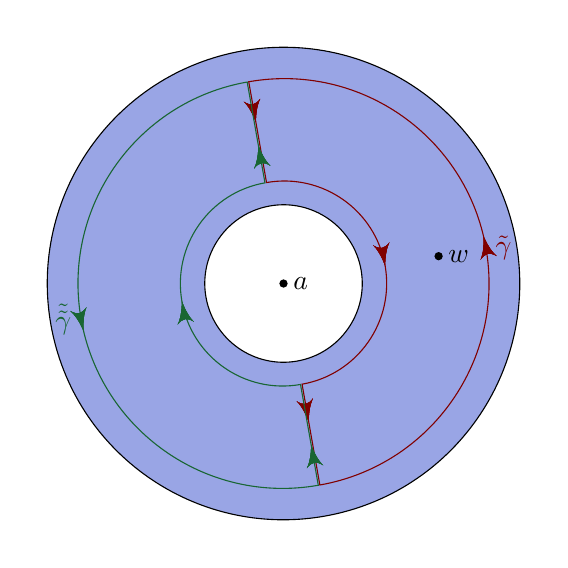
\begin{tikzpicture}[rotate=10]
      \draw [fill opacity=0.5, fill=mblue] circle [radius=3];
      \draw [fill=white] circle [radius=1];

      \node at (0, 0) [right] {$a$};
      \node [circ] at (0, 0) {};

      \draw [mred, ->-=0, ->-=0.17, ->-=0.51, ->-=0.81] (1.31, 0) arc(0:-90:1.3) -- (0.01, -2.6) arc(-90:90:2.6) node [pos=0.5, right] {$\tilde{\gamma}$} -- (0.01, 1.3) arc(90:0:1.3);
      \draw [mgreen, ->-=0, ->-=0.17, ->-=0.51, ->-=0.81] (-1.31, 0) arc(180:90:1.3) -- (-0.01, 2.6) arc(90:270:2.6) node [pos=0.5, left] {$\tilde{\tilde{\gamma}}$} -- (-0.01, -1.3) arc(270:180:1.3);

      \node [circ] at (2, 0) {};
      \node [right] at (2, 0) {$w$};
    \end{tikzpicture}
  \end{center}
  We let $\tilde{\gamma}$ be the contour containing $w$, and $\tilde{\tilde{\gamma}}$ be the other contour.

  Now we apply the Cauchy integral formula to say
  \[
    f(w) = \frac{1}{2\pi i} \int_{\tilde{\gamma}}\frac{f(z)}{z - w}\;\d z
  \]
  and
  \[
    0 = \frac{1}{2\pi i} \int_{\tilde{\tilde{\gamma}}} \frac{f(z)}{z - w} \;\d z.
  \]
  So we get
  \[
    f(w) = \frac{1}{2\pi i} \int_{\partial B(a, \rho'')} \frac{f(z)}{z - w}\;\d z - \frac{1}{2\pi i} \int_{\partial B(a, \rho')} \frac{f(z)}{z - w}\;\d z.
  \]
  As in the first proof of the Cauchy integral formula, we make the following expansions: for the first integral, we have $w - a < z - a$. So
  \[
    \frac{1}{z - w} = \frac{1}{z - a} \left(\frac{1}{1 - \frac{w - a}{z - a}}\right) = \sum_{n = 0}^\infty \frac{(w - a)^n}{(z - a)^{n + 1}},
  \]
  which is uniformly convergent on $z \in \partial B(a, \rho'')$.

  For the second integral, we have $w - a> z - a$. So
  \[
    \frac{-1}{z - w} = \frac{1}{w - a} \left(\frac{1}{1 - \frac{z - a}{w - a}}\right) = \sum_{m = 1}^\infty \frac{(z - a)^{m - 1}}{(w - a)^m},
  \]
  which is uniformly convergent for $z \in \partial B(a, \rho')$.

  By uniform convergence, we can swap summation and integration. So we get
  \begin{align*}
    f(w) ={}& \sum_{n = 0}^\infty \left(\frac{1}{2 \pi i} \int_{\partial B(a, \rho'')} \frac{f(z)}{(z - a)^{n + 1}} \;\d z\right) (w - a)^n \\
    &+ \sum_{m = 1}^\infty \left(\frac{1}{2\pi i} \int_{\partial B(a, \rho')}\frac{f(z)}{(z - a)^{-m + 1}} \;\d z\right) (w - a)^{-m}.
  \end{align*}
  Now we substitute $n = -m$ in the second sum, and get
  \[
    f(w) = \sum_{n = -\infty}^\infty \tilde{c}_n (w - a)^n,
  \]
  for the integrals $\tilde{c}_n$. However, some of the coefficients are integrals around the $\rho''$ circle, while the others are around the $\rho'$ circle. This is not a problem. For any $r < \rho < R$, these circles are convex deformations of $|z - a| = \rho$ inside the annulus $A$. So
  \[
    \int_{\partial B(a, \rho)} \frac{f(z)}{(z - a)^{n + 1}} \;\d z
  \]
  is independent of $\rho$ as long as $\rho \in (r, R)$. So we get the result stated.
\end{proof}

\begin{defi}[Principal part]
  If $f: B(a, r)\setminus \{a\} \to \C$ is holomorphic and if $f$ has Laurent series
  \[
    f(z) = \sum_{n = -\infty}^\infty c_n (z - a)^n,
  \]
  then the \emph{principal part} of $f$ at $a$ is
  \[
    f_{\mathrm{principal}} = \sum_{n = -\infty}^{-1} c_n (z - a)^n.
  \]
\end{defi}
So $f - f_{\mathrm{principal}}$ is holomorphic near $a$, and $f_{\mathrm{principal}}$ carries the information of what kind of singularity $f$ has at $a$.

When we talked about Taylor series, if $f: B(a, r) \to \C$ is holomorphic with Taylor series $f(z) = \sum_{n = 0}^\infty c_n(z - a)^n$, then we had two possible ways of expressing the coefficients of $c_n$. We had
\[
  c_n = \frac{1}{2\pi i} \int_{\partial B(a, \rho)} \frac{f(z)}{(z - a)^{n + 1}}\;\d z = \frac{f^{(n)}(a)}{n!}.
\]
In particular, the second expansion makes it obvious the Taylor series is uniquely determined by $f$.

For the Laurent series, we cannot expect to have a simple expression of the coefficients in terms of the derivatives of the function, for the very reason that $f$ is not even defined, let alone differentiable, at $a$. So is the Laurent series unique?

\begin{lemma}
  Let $f: A \to \C$ be holomorphic, $A = \{r < |z - a| < R\}$, with
  \[
    f(z) = \sum_{n = -\infty}^{\infty} c_n(z - a)^n
  \]
  Then the coefficients $c_n$ are uniquely determined by $f$.
\end{lemma}

\begin{proof}
  Suppose also that
  \[
    f(z) = \sum_{n = -\infty}^\infty b_n (z - a)^n.
  \]
  Using our formula for $c_k$, we know
  \begin{align*}
    2\pi i c_k &= \int_{\partial B(a, \rho)} \frac{f(z)}{(z - a)^{k + 1}} \;\d z \\
    &= \int_{\partial B(a, \rho)} \left(\sum_n b_n (z - a)^{n - k - 1}\right)\;\d z\\
    &= \sum_n b_n \int_{\partial B(a, \rho)} (z - a)^{n - k - 1}\;\d z\\
    &= 2\pi i b_k.
  \end{align*}
  So $c_k = b_k$.
\end{proof}
While we do have uniqueness, we still don't know how to find a Laurent series. For a Taylor series, we can just keep differentiating and then get the coefficients. For Laurent series, the above integral is often almost impossible to evaluate. So the technique to compute a Laurent series is blind guesswork.

\begin{eg}
  We know
  \[
    \sin z = z - \frac{z^3}{3!} + \frac{z^5}{5!} - \cdots
  \]
  defines a holomorphic function, with a radius of convergence of $\infty$. Now consider
  \[
    \cosec z = \frac{1}{\sin z},
  \]
  which is holomorphic except for $z = k\pi$, with $k \in \Z$. So $\cosec z$ has a Laurent series near $z = 0$. Using
  \[
    \sin z = z\left(1 - \frac{z^2}{6} + O(z^4)\right),
  \]
  we get
  \[
    \cosec z = \frac{1}{z} (1 + \frac{z^2}{6} + O(z^4).
  \]
  From this, we can read off that the Laurent series has $c_n = 0$ for all $n \leq -2$, $c_{-1} = 1$, $c_1 = \frac{1}{5}$. If we want, we can go further, but we already see that $\cosec$ has a simple pole at $z = 0$.

  By periodicity, $\cosec$ has a simple pole at all other singularities.
\end{eg}

\begin{eg}
  Consider instead
  \[
    \sin \left(\frac{1}{z}\right) = \frac{1}{z} - \frac{1}{3! z^3} + \frac{1}{5! z^5} - \cdots.
  \]
  We see this is holomorphic on $\C^*$, with $c_n \not= 0$ for infinitely many $n < 0$. So this has an isolated essential singularity.
\end{eg}

\begin{eg}
  Consider $\cosec \left(\frac{1}{z}\right)$. This has singularities at $z = \frac{1}{k\pi}$ for $k \in \N = \{1, 2, 3, \cdots\}$. So it is not holomorphic at any punctured neighbourhood $B(0, r)\setminus \{0\}$ of zero. So this has a \emph{non-isolated} singularity at zero, and there is \emph{no} Laurent series in a neighbourhood of zero.
\end{eg}

From now on, the course will involve applying the techniques we've developed so far to some seemingly unrelated fields. One of the classical applications is to evaluate some series.
\begin{eg}[Series summation]
  We claim that
  \[
    f(z) = \sum_{n = -\infty}^\infty \frac{1}{(z - n)^2}
  \]
  is holomorphic on $\C \setminus \Z$, and moreover
  \[
    f(z) = \frac{\pi^2}{\sin^2(\pi z)}.
  \]
  For $w \in \C\setminus \Z$, we use comparison to $\sum \frac{1}{n^2}$. We pick $r > 0$ such that $|w - n| > 2r$ for all $n \in \Z$. Then for all $z \in B(w; r)$, we have
  \[
    |z - n| \geq \max\{r, n - |w| - r\}.
  \]
  Hence
  \[
    \frac{1}{|z - n|^2} \leq \min\left\{\frac{1}{r^2}, \frac{1}{(n - |w| - r)^2}\right\} = M_n.
  \]
  By comparison to $\sum \frac{1}{n^2}$, we know $\sum_n M_n$ converges. So by the Weierstrass $M$-test, we know our series converges uniformly on $B(w, r)$.

  By our results around Morera's theorem, we see that $f$ is a uniform limit of holomorphic functions $\sum_{n = -N}^N \frac{1}{(z - n)^2}$, and hence holomorphic.

  Since $w$ was arbitrary, we know $f$ is holomorphic on $\C \setminus \Z$. Note that we do not say the sum converges uniformly on $\C \setminus \Z$. It's just that for any point $w \in \C \setminus \Z$, there is a small neighbourhood of $w$ on which the sum is uniformly convergent, and this is sufficient to apply the result of Morera's.

  For the second part, note that $f$ is periodic, since $f(z + 1) = f(z)$. Also, at $0$, $f$ has a double pole, since $f(z) = \frac{1}{z^2} + $ holomorphic stuff near $z = 0$. So $f$ has a double pole at each $k \in \Z$. Note that $\frac{1}{\sin^2 (\pi z)}$ also has a double pole at each $k \in \Z$.

  Now, consider the principal parts of our functions --- at $k \in \Z$, $f(z)$ has principal part $\frac{1}{(z - k)^2}$. Looking at our previous Laurent series for $\cosec (z)$, if
  \[
    g(z) = \left(\frac{\pi}{\sin \pi z}\right)^2,
  \]
  then $\lim_{z \to 0} z^2 g(z) = 1$. So $g(z)$ must have the same principal part at $0$ and hence at $k$ for all $k \in \Z$.

  Hence $h(z) = f(z) - g(z)$ is holomorphic on $\C \setminus \Z$. However, since its principal part vanishes at the integers, it has at worst a removable singularity. Removing the singularity, we know $h(z)$ is entire.

  Since we want to prove $f(z) = g(z)$, we need to show $h(z) = 0$. To do this, we only have to show it is bounded and vanishes at a point, by Liouville's theorem.

  We first show boundedness. We know $f$ and $g$ are both periodic with period $1$. So it is natural to focus attention on the strip $-\frac{1}{2} \leq x = \Re(z) \leq \frac{1}{2}$.

  If we further focus on the rectangle $x \in [-\frac{1}{2}, \frac{1}{2}]$, $y \in [-Y, Y]$, then we get a bound from the continuity on $h$ on a closed bounded set. Finally, for $z = x + iy$, $|x| \leq \frac{1}{2}$, wlog $y > 0$, we bound $f$ and $g$ separately for large $y$: we have
  \[
    |g(z)| \leq \frac{4\pi^2}{|e^{\pi y} - e^{- \pi y}|} \to 0
  \]
  as $y \to \infty$. Exactly analogously,
  \[
    |f(z)| \leq \sum_{n \in \Z} \frac{1}{|x + iy - n|^2} \leq \frac{1}{y^2} + 2 \sum_{n = 1}^\infty \frac{1}{(n - \frac{1}{2})^2 + y^2} \to 0
  \]
  as $y \to \infty$. So $h$ is bounded on the strip, and tends to $0$ as $y \to \infty$, and is hence constant by Liouville's theorem. But if $h \to 0$ as $y \to \infty$, then the constant better be zero. So we get
  \[
    h(z) = 0.
  \]
\end{eg}

\section{Residue calculus}
\subsection{Winding numbers}
Recall that the integral of a curve around a singularity tells us something about the singularity, via the Laurent series and the Cauchy integral formula. This allows us to deal with cases with exactly one singularity and rather simple curves. To deal with more complicated objects, we need some more definitions.

\begin{defi}[Residue]
  Let $f: B (a, r) \setminus \{a\} \to \C$ be holomorphic, with Laurent series
  \[
    f(z) = \sum_{n = -\infty}^\infty c_n (z - a)^n.
  \]
  Then the \emph{residue} of $f$ at $a$ is
  \[
    \Res(f, a) = \Res_f(a) = c_{-1}.
  \]
\end{defi}
Note that if $\rho < r$, then we have
\[
  \int_{\partial \overline{B(a, \rho)}} f(z)\;\d z = 2\pi i c_{-1}.
\]
So we can alternatively write
\[
  \Res_f(a) = \frac{1}{2 \pi i}\int_{\partial \overline{B(a, \rho)}} f(z)\;\d z.
\]
This gives us a formulation of the residue without reference to the Laurent series.

However, consider non-simple a $C^1$ curve $\gamma$ as shown below:
\begin{center}
  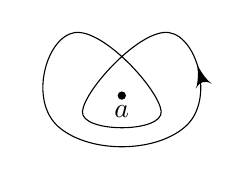
\begin{tikzpicture}
    \draw [->-=0.45] plot [smooth cycle, tension=1] coordinates {(0.5, -1) (-0.6, 0) (-0.8, -1.2) (0.8, -1.2) (0.6, 0) (-0.5, -1)};
    \node [circ] at (0, -0.8) {};
    \node [below] at (0, -0.8) {$a$};
  \end{tikzpicture}
\end{center}
by the additivity of the integral, we can break this curve into two closed contours, and then we know
\[
  \frac{1}{2\pi i} \int_\gamma f(z)\;\d z = 2 \Res_f(a).
\]
We obtained the coefficient $2$ by looking at the curve and trying to chop it up into two. However, while this works for this particular case, it is difficult to formalize and generalize. We want more generally a notion of how a given closed curve (not necessarily simple) winds around a point $a$ not lying on the curve.

\begin{lemma}
  Let $\gamma: [a, b] \to \C$ be a continuous closed curve, and let $w \in \C \setminus \image (\gamma)$. Then there are continuous functions $r: [a, b] \to \R \geq 0$ and $\theta: [a, b] \to \R$ such that
  \[
    \gamma(t) = w + r(t) e^{i\theta(t)}.
  \]
\end{lemma}
Of course, at each point $t$, we can find $r$ and $\theta$ such that the above holds. The key point of the lemma is that we can do so continuously.

\begin{proof}
  Clearly $r(t) = |\gamma(t) - w|$ exists and is continuous, since it is the composition of continuous functions. Note that this is never zero since $\gamma(t)$ is never $w$. The actual content is in defining $\theta$.

  To define $\theta(t)$, we for simplicity assume $w = 0$. Furthermore, by considering instead the function $\frac{\gamma(t)}{r(t)}$, which is continuous and well-defined since $r$ is never zero, we can assume $|\gamma(t)| = 1$ for all $t$.

  Recall that the principal branch of $\log$, and hence of the argument $\Im (\log)$, takes values in $(-\pi, \pi)$ and is defined on $\C \setminus \R_{\leq 0}$.
  \begin{center}
    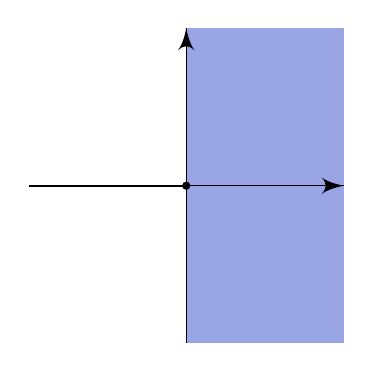
\begin{tikzpicture}
      \fill [mblue, opacity=0.5] (0, 2) rectangle (2, -2);
      \draw [->] (0, 0) -- (2, 0);
      \draw [thick] (-2, 0) -- (0, 0);
      \draw [->] (0, -2) -- (0, 2);
      \node [circ] at (0, 0) {};
    \end{tikzpicture}
  \end{center}
  If $\gamma(t)$ always lied in, say, the right-hand half plane, we would have no problem defining $\theta$ consistently, since we can just let
  \[
    \theta(t) = \arg(\gamma(t))
  \]
  for $\arg$ the principal branch. There is nothing special about the right-hand half plane. Similarly, if $\gamma$ lies in the region as shaded below:
  \begin{center}
    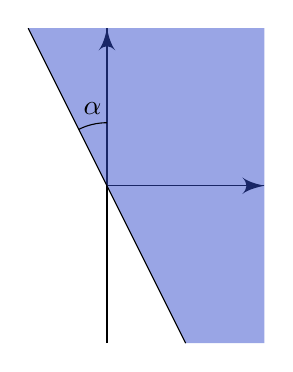
\begin{tikzpicture}
      \draw [->] (0, 0) -- (2, 0);
      \draw [->] (0, -2) -- (0, 2);

      \fill [mblue, opacity=0.5] (-1, 2) -- (1, -2) -- (2, -2) -- (2, 2) -- cycle;
      \draw (-1, 2) -- (1, -2);

      \draw (0, 0.8) arc(90:116.56:0.8) node [pos=0.5, above] {$\alpha$};
    \end{tikzpicture}
  \end{center}
  ie. we have
  \[
    \gamma(t) \in \left\{z : \Re\left(\frac{z}{e^{i\alpha}}\right) > 0\right\}
  \]
  for a fixed $\alpha$, we can define
  \[
    \theta(t) = \alpha + \arg\left(\frac{\gamma(t)}{e^{i\alpha}}\right).
  \]
  Since $\gamma: [a, b] \to \C$ is continuous, it is uniformly continuous, and we can find a subdivision
  \[
    a = a_0 < a_1 < \cdots < a_m = b,
  \]
  such that if $s, t \in [a_{i - 1}, a_i]$, then $|\gamma(s) - \gamma(t)| < \sqrt{2}$, and hence $\gamma(s)$ and $\gamma(t)$ belong to such a half-plane.

  So we define $\theta_j: [a_{j - 1}, a_j] \to \R$ such that
  \[
    \gamma(t) = e^{i\theta_j(t)}
  \]
  for $t \in [a_{j - 1}, a_j]$, and $1 \leq j \leq n - 1$.

  What happens at the boundary? We know $\theta_j(a_j)$ and $\theta_{j + 1}(a_j)$ are both values of the argument for a fixed complex number, hence differ by an element of $2\pi \Z$.

  Now, for $j > 1$, we can successively re-define $\theta_j$ such that the resulting map $\theta$ is continuous, by shifting the individual $\theta_j$'s by integer multiples of $2\pi$. So done.
\end{proof}
This allows us to define the winding number by considering how $\theta$ varies along the path.

\begin{defi}[Winding number]
  Given a continuous path $\gamma: [a, b] \to \C$ such that $\gamma(a) = \gamma(b)$ and $w \not\in \image(\gamma)$, the \emph{winding number} of $\gamma$ about $w$ is
  \[
    \frac{\theta(b) - \theta(a)}{2\pi},
  \]
  where $\theta: [a, b] \to \R$ is a continuous function as above. This is denoted by $I(\gamma, w)$ or $n_\gamma(W)$.
\end{defi}
$I$ and $n$ stand for index and number respectively.

Note that we always have $I(\gamma, w) \in \Z$, since $\theta(b)$ and $\theta(a)$ are arguments of the same number. More importantly, $I(\gamma, w)$ is well-defined --- suppose $\gamma(t) = r(t) e^{i \theta_1(t)} = r(t) e^{i\theta_2(t)}$ for continuous functions $\theta_1, \theta_2: [a, b] \to \R$. Then $\theta_1 - \theta_2 : [a, b] \to \R$ is continuous, but takes values in the discrete set $2\pi \Z$. So it must in fact be constant, and thus $\theta_1(b) - \theta_1(a) = \theta_2(b) - \theta_2(a)$.

So far, what we've done is something that is true for arbitrary continuous closed curve. However, if we focus on piecewise $C^1$-smooth closed path, then we get an alternative expression:
\begin{lemma}
  Suppose $\gamma: [a, b] \to \C$ is a piecewise $C^1$-smooth closed path, and $w \not\in \image(\gamma)$. Then
  \[
    I(\gamma, w) = \frac{1}{2\pi i} \int_\gamma \frac{1}{z - w} \;\d z.
  \]
\end{lemma}

\begin{proof}
  Let $\gamma(t) - w = r(t) e^{i \theta(t)}$, with now $r$ and $\theta$ piecewise $C^1$-smooth. Then
  \begin{align*}
    \int_\gamma \frac{1}{z - w}\;\d z &= \int_a^b \frac{\gamma'(t)}{\gamma(t) - w}\;\d t\\
    &= \int_a^b \left(\frac{r'(t)}{r(t)} + i \theta'(t)\right) \;\d t\\
    &= [\ln r(t) + i\theta(t)]^b_a\\
    &= i(\theta(b) - \theta(a))\\
    &= 2\pi i I(\gamma, w).
  \end{align*}
  So done.
\end{proof}

In some books, this integral expression is taken as the definition of the winding number. While this is elegant in complex analysis, it is not clear \emph{a priori} that this is an integer, and only works for piecewise $C^1$-smooth closed curves, not arbitrary continuous closed curves.

On the other hand, what is evident from this expression is that $I(\gamma, w)$ is continuous as a function of $w \in \C \setminus \image(\gamma)$, since it is even holomorphic as a function of $w$. Since $I(\gamma; w)$ is integer valued, $I(\gamma)$ must be locally constant on path components of $\C \setminus \image(\gamma)$.

Also, since $\image(\gamma)$ is compact, all points of sufficiently large modulus in $\C$ belong to one component of $\C \setminus \image(\gamma)$. This is indeed the only path component of $\C\setminus \image(\gamma)$ that is unbounded. This is a distinguished path component of $\C \setminus \image(\gamma)$. So the winding number has a distinguished value at this unbounded component. Fortunately, this is zero.

Indeed, as $I(\gamma; w)$ is consistent on this component, we can consider arbitrarily larger $w$. By the integral formula,
\[
  |I(\gamma, w)| \leq \frac{1}{2\pi} \length(\gamma) \max_{z \in \gamma} \frac{1}{|w - z|} \to 0
\]
as $w \to \infty$. However, inside the other path components, we can still have some interesting values of the winding number.

\subsection{The Cauchy residue theorem}
We are now going to obtain a more general version of Cauchy's theorem. This will involve the idea of winding numbers. This will also need the idea of curves being homotopic.
\begin{defi}[Homotopy of closed curves]
  Let $U \subseteq \C$ be a domain, and let $\phi: [a, b] \to U$ and $\psi: [a, b] \to U$ be piecewise $C^1$-smooth closed paths. A \emph{homotopy} from $\phi: \psi$ is a continuous map $F: [0, 1] \times [a, b] \to U$ such that
  \[
    F(0, t) = \phi(t),\quad F(1, t) = \psi(t),
  \]
  and moreover, for all $s \in [0, t]$, the map $t \mapsto F(s, t)$ viewed as a map $[a, b] \to U$ is closed and piecewise $C^1$-smooth.
\end{defi}
We can imagine this as a process of ``continuously deforming'' the path $\phi$ to $\psi$, with a path $F(s, \ph)$ at each point in time $s \in [0, 1]$.

Recall from long time ago that we have the notion of a convex deformation --- given $\phi, \psi: [a, b] \to U$, which are closed, we say $\psi$ is an \emph{elementary deformation} or \emph{convex deformation} of $\phi$ if there exists a decomposition $a = x_0 < x_1 < \cdots < x_n = b$ and convex open sets $C_1, \cdots, C_n \subseteq U$ such that for $x_{i - 1} \leq t \leq x_i$, we have $\phi(t)$ and $\psi(t)$ in $C_i$. Let $\gamma_i \subseteq C_i$ be the straight path from $\phi(x_i)$ to $\psi(x_i)$.

Then if $f: U \to \C$ is holomorphic, we claimed that
\[
  \int_\phi f(x)\;\d z = \int_\psi f(z)\;\d z.
\]
This is since we can let $\phi_i = \phi|_{[x_{i - 1}, x_i]}$, and similarly for $\psi$ and then by the convex Cauchy theorem, we know
\[
  \int_{\phi_i + \gamma_i - \psi_i - \gamma_{i - 1}} f(z)\;\d z = 0.
\]
Summing this over all $i$, we obtain the required identity.

While the definition of elementary deformation allowed us to prove this property with ease, the definition itself is unnatural and weird. We have to make reference to this arbitrarily constructed dissection of $[a, b]$ and convex sets $C_i$. Moreover, this rigid definition of elementary definition fails to be transitive (exercise). % fill
Homotopy is a much more natural definition to use, and is easily seen to be an equivalence relation. Fortunately, we have the following proposition:

\begin{prop}
  Let $\phi, \psi: [a, b] \to U$ be homotopic (piecewise $C^1$) closed paths in a domain $U$. Then there exists some $\phi = \phi_0, \phi_1, \cdots, \phi_N = \psi$ such that each $\phi_j$ is piecewise $C^1$ closed and $\phi_{i + 1}$ is obtained from $\phi_i$ by elementary deformation.
\end{prop}

\begin{proof}
  This is an exercise in uniform continuity. We let $F: [0, 1] \times [a, b] \to U$ be a homotopy from $\phi$ to $\psi$. Since $\image (F)$ is compact and $U$ is open, there is some $\varepsilon > 0$ such that $B(F(s, t), \varepsilon) \subseteq U$ for all $(s, t) \in [0, 1] \times [a, b]$ (for each $s, t$, there is an $\varepsilon_{s, t}$ such that $B(F(s, t), \varepsilon_{s, t}) \subseteq U$, and by compactness, finitely many of these balls cover $\image(F)$. Then taking the minimum of all these $\varepsilon_{s, t}$ gives the desired $\varepsilon$).

  Since $F$ is uniformly continuous, there is some $\delta$ such that $\|(s, t) - (s', t')\| < \delta$ implies $|F(s, t) - F(s', t')| < \varepsilon$.

  Now we pick $n \in \N$ such that $\frac{1 + (b - a)}{n} < \delta$, and let
  \begin{align*}
    x_j &= a + (b - a) \frac{j}{n}\\
    \phi_i(t) &= F\left(\tfrac{i}{n}, t\right)\\
    C_{ij} &= B\left(F\left(\tfrac{i}{n}, x_j\right), \varepsilon\right)
  \end{align*}
  Then $C_{ij}$ is clearly convex. These definitions are cooked up precisely so that if $s \in \left(\frac{i - 1}{n}, \frac{i}{n}\right)$ and $t \in [x_{j - 1}, x_j]$, then $F(s, t) \in C_{ij}$. So the result follows.
\end{proof}
So homotopies are sequences of elementary deformations, and elementary deformations don't change integrals.

We can now ``upgrade'' our Cauchy integral formula. We first re-define what it means for a domain to be simply connected:
\begin{defi}[Simply connected domain]
  A domain $U$ is \emph{simply connected} if every $C^1$ smooth closed path is homotopic to a constant path.
\end{defi}
This is in fact equivalent to our earlier definition that every continuous map $S^1 \to U$ can be extended to a continuous map $D^2 \to U$. This is almost immediately obvious, except that our old definition only required the map to be continuous, while the new definition only works with piecewise $C^1$ paths. We will need something that allows us to approximate any continuous curve with a piecewise $C^1$-smooth one, but we shall not do that here. Instead, we will just forget about the old definition and stick to the new one.

\begin{cor}
  Let $U$ be a domain, $f: U \to \C$ be holomorphic, and $\gamma_1, \gamma_2$ be homotopic piecewise $C^1$-smooth closed curves in $U$. Then
  \[
    \int_{\gamma_1}f(z)\;\d z = \int_{\gamma_2}f(z)\;\d z.
  \]
\end{cor}
This means the integral around any path depends only on the homotopy class of the path, and not the actual path itself.

This then implies
\begin{cor}[Cauchy's theorem for simply connected domains]
  Let $U$ be a simply connected domain, and let $f: U \to \C$ be holomorphic. If $\gamma$ is any piecewise $C^1$-smooth closed curve in $U$, then
  \[
    \int_\gamma f(z)\;\d z = 0.
  \]
\end{cor}

\begin{proof}
  By definition of simply-connected, $\gamma$ is homotopic to the constant path, and it is easy to see the integral along a constant path is zero.
\end{proof}

Recall we also had the Cauchy integral formula. If $f: B(a, r) \to \C$ is holomorphic, $w \in B(a, \rho)$ and $\rho < r$, then
\[
  f(w) = \frac{1}{2\pi i} \int_{\partial \overline{B(a, \rho)}} \frac{f(z)}{z - w}\;\d z.
\]
This is a version of Cauchy's theorem where $g: U \to \C$ is holomorphic only $U\setminus \{w\}$, with $g(z) = \frac{f(z)}{z - w}$.

The idea is that if the function $g$ is not holomorphic at $w$, then we pick up a non-zero value as we go around the point $w$.

The following result is a powerful generalization of these ideas:
\begin{thm}[Cauchy's Residue theorem]
  Let $U$ be a simply connected domain, and let $\{z_1, \cdots, z_k\} \subseteq U$, and let $f: U \setminus \{z_1, \cdots, z_k\} \to \C$ be holomorphic. Let $\gamma: [a, b] \to U$ be a piecewise $C^1$-smooth closed curve such that $z_i \not= \image(\gamma)$ for all $i$. The
  \[
    \frac{1}{2\pi i} \int_{\gamma}f(z)\;\d z = \sum_{j = 1}^k I(\gamma, z_i) \Res(f; z_i).
  \]
\end{thm}
The Cauchy integral formula and simply-connected Cauchy are special cases of this.

\begin{proof}
  At $z_i$, $f$ has a Laurent expansion
  \[
    f(z) = \sum_{n \in \Z} c_n^{(i)} (z - z_i)^n,
  \]
  valid in some neighbourhood of $z_i$. Let $g_i(z)$ be the principal part, namely
  \[
    g_i(z) = \sum_{n = -\infty}^{-1} c_n^{(i)}(z - z_i)^n.
  \]
  From the proof of the Laurent series, we know $g_i(z)$ gives a holomorphic function on $U \setminus \{z_i\}$.

  We now consider $f - g_1 - g_2 - \cdots - g_k$, which is holomorphic on $U \setminus \{z_1, \cdots, z_k\}$, and has a \emph{removable} singularity at each $z_i$. So
  \[
    \int_\gamma (f - g_1 - \cdots - g_k)(z)\;\d z = 0,
  \]
  by simply-connected Cauchy. Hence we know
  \[
    \int_\gamma f(z)\;\d z = \sum_{j = 1}^k \int_\gamma g_j(z)\;\d z.
  \]
  For each $j$, we use uniform convergence of the series $\sum_{n \leq -1} c_n^{(j)} (z - z_j)^n$ on compact subsets of $U \setminus \{z_j\}$, and hence on $\gamma$, to write
  \[
    \int_\gamma g_j(z)\;\d z = \sum_{n \leq -1} c_n^{(j)} \int_\gamma (z - z_j)^n\;\d z.
  \]
  However, for $n \not= -1$, the function $(z - z_j)^n$ has an antiderivative, and hence the integral around $\gamma$ vanishes. So this is equal to
  \[
    c_{-1}^{(j)} \int_\gamma \frac{1}{z - z_j}\;\d z.
  \]
  But $c_{-1}^{(j)}$ is by definition the residue of $f$ at $z_j$, and the integral is just the integral definition of the winding number (up to a factor of $2\pi i$). So we get
  \[
    \int_\gamma f(z)\;\d z = 2\pi i \sum_{j = 1}^k \Res(f; z_j) I(\gamma, z_j).
  \]
  So done.
\end{proof}


\end{document}
